\documentclass{article}

\usepackage[utf8]{inputenc}
\usepackage{graphicx}
\usepackage{url}
\usepackage{color}
\usepackage{titlesec}
\usepackage{amsmath}
\usepackage{physics}
\usepackage{amsfonts}
\usepackage{subcaption}
\usepackage{booktabs}
\usepackage[counterclockwise]{rotating}
\graphicspath{{../figures/}}

\title{Cleaned up first paper draft for supersat project}
\author{K. Latimer}
\date{Dec 30, 2020}

\newcommand{\drcomm}[1]{\textcolor{blue}{\textit{#1}}}
\newcommand{\klcomm}[1]{\textcolor{red}{\textit{#1}}}

\begin{document}

\maketitle

\noindent\drcomm{Questions/comments from DR in blue} \\
\noindent\klcomm{Responses from KL in red}\\

\section{Intro}

In a recent paper, Fan et al introduce a novel ``warm phase invigoration mechanism" (WPIM) in which increased concentrations of ultrafine aerosol particles (UAP$_{<50}$, with 50 signifying an upper bound on particle diameter of 50nm) in the boundary layer (BL) result in enhanced convective updraft speeds and precipitation rates \cite{Fan2018}. As pointed out by Grabowski and Morrison, the precise explanation for this physical effect is that, in allowing for lower equilibrium water vapor supersaturation (SS) values in rising convective parcels, these excess aerosol particles lead to an increase in the buoyancy of the parcel over the course of its ascent, thus enhancing convective speeds \cite{Grabowski2020}.

In order to get a quantitative intuition for how this works, we offer a simplified version of the calculation in \cite{Grabowski2015}, which still conveys the same essential idea. We consider a polluted (non-supersaturated; i.e. $RH=1$) storm ascending in an environment whose temperature profile has been set by clean storms. The parcel condenses water vapor as it rises, and for simplicity we assume no latent heat is lost to the environment. We then have (see Table \ref{vartable} for explanation of constants and variables used in the text. We use $\delta$ here to represent a variation in state variables between two parcels, as distinguised from $d$ in Equation \ref{dCAPE} which denotes a proper differential form):
\begin{equation}
\label{energyconsv}
C_{ap}\delta T + L_v\delta q_v = 0,
\end{equation}
where $q_v$ is the water vapor mass fraction of the parcel ($q_v=m_v/m_{tot}$), also expressed in terms of the the relative humidity ($RH$) and saturation water vapor mass fraction ($q_v^*$) as:
\begin{equation}
\label{qveqn}
q_v = RHq_v^*
\end{equation}
Usig the Clausius-Clayperon equation:
\begin{align}
\label{clauclay}
\delta q_v^* &= \delta \Big(\frac{e_sV}{R_vTm_{tot}}\Big)\nonumber\\ 
&=\frac{\delta e_s}{e_s}q_v^* - \frac{\delta T}{T}q_v^*\nonumber\\ 
&=\frac{L_v\delta T}{R_vT^2}q_v^* - \frac{\delta T}{T}q_v^*\nonumber\\ 
&=\Big(\frac{L_v}{R_vT} - 1\Big)\frac{\delta T}{T}q_v^*\nonumber\\ 
&\approx \frac{q_v^*L_v}{R_vT^2}\delta T 
\end{align}
Taking the differential of Equation \ref{qveqn} and rearranging terms in Equations \ref{energyconsv}, \ref{qveqn}, and \ref{clauclay} yields:
\begin{equation}
\label{dT}
\delta T = \frac{-L_vq_v^*}{C_{pa} + q_v\frac{L_v^2}{R_vT^2}}\delta RH
\end{equation}
Plugging in typical values for $RH$ ($\approx 1.1$) and $T$ ($\approx 300$ K) gives $dT\approx 1$ K.

In their paper (see for example Figure 2(b) of that work), Fan et al provide anecdotal evidence that the WPIM is capable of producing enhancements in vertical wind velocity on the order of 10 m/s for polluted relative to unpolluted storms. Even neglecting diffusive, frictional, or radiative losses, this requires a variation in convective available potential energy ($CAPE$) of $\approx 100$ J/kg, or a $RH$ difference between the dirty storm and clean environment of $\approx 0.1$, i.e., the environment must support SS on the order of 10\% throughout the troposphere.

While Fan et al do not offer any proof based on experimental data that such high SS exist in the convection setting the environmental lapse rate, they do observe comparable values in numerical simulations. In particular, using the Weather Research and Forcasting (WRF) model to simulate pristine (no UAP$_{<50}$) conditions in the Amazon Rainforest, they find (horizontally- and time-averaged) SS in convective cores of up to 15\%.

Since this is well above what is typically reported or assumed in the literature [ \klcomm{TODO - find some citations} ], we seek in this paper to determine if we can find experimental evidence for O(10\%) SS in nature. We use data from the High-Altitude LOng-range research aircraft (HALO) (part of the ACRIDICON-CHUVA mission in and around Manaus, Brazil in 2014-15), as well as from the first phase of the Cloud Aerosol Interaction and Precipitation Enhancement EXperiment (CAIPEEX) in India (taken in June [around Hyderabad] and August [around Bareilly] 2009) \cite{???, Kulkarni2012} as a dataset of opportunity.

\section{Data Analysis and Results}

In order to determine experimental supersaturation within a reasonable margin of error, we must use the quasi-steady-state (QSS) supersaturation formula \cite{Rogers1989}. Based on our analysis of the WRF data, this approximation is only valid within certain limits, namely:
\begin{itemize}
	\item T \textgreater  273K (we're not including ice in the theory; note that Fan et al do evaluate SS wrt water above the freezing line though)
	\item w \textgreater  2 m/s (reasonably strong updrafts)
	\item cloud LWC \textgreater  1e-4 g/g (in the convection core)
	\item including rain droplets and ventillation corrections
\end{itemize}

Figure \ref{wrfvsqss} shows a scatterplot with the agreement between the actual and QSS-derived SS values in the WRF simulation, for points satisfying the above criteria. For brevity we will henceforth refer to such points as `cloudy updrafts.'

\clearpage
\newpage

\begin{figure}[ht]
	\centering
	\begin{subfigure}{0.7\textwidth}
		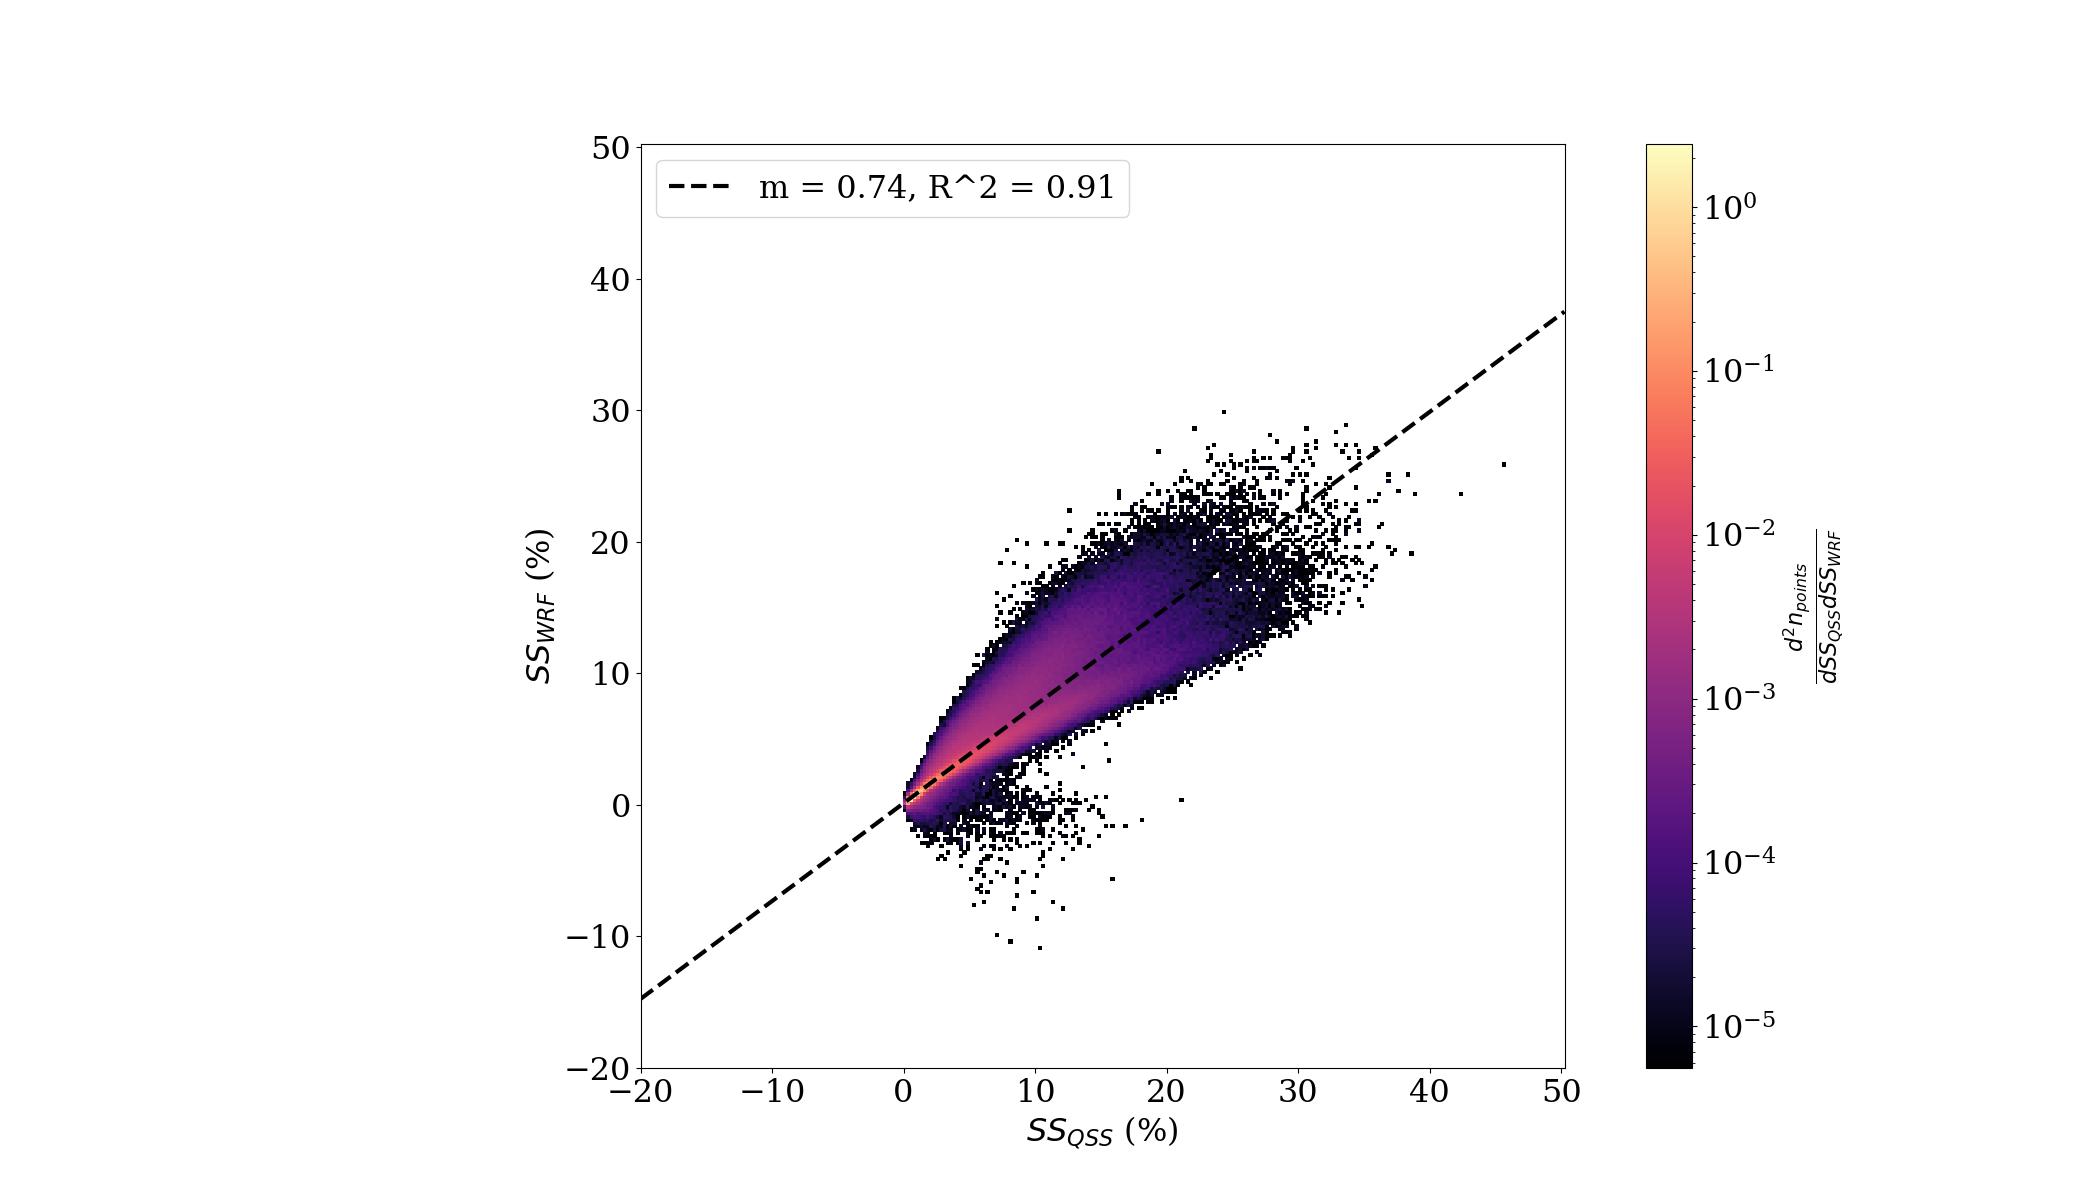
\includegraphics[width=\textwidth]{revmywrf/v1_FINAL_heatmap_ss_qss_vs_ss_wrf_Unpolluted_figure.png}
		\caption{Unpolluted case.}
		\label{wrfvsqssunpoll}
	\end{subfigure}
	\begin{subfigure}{0.7\textwidth}
		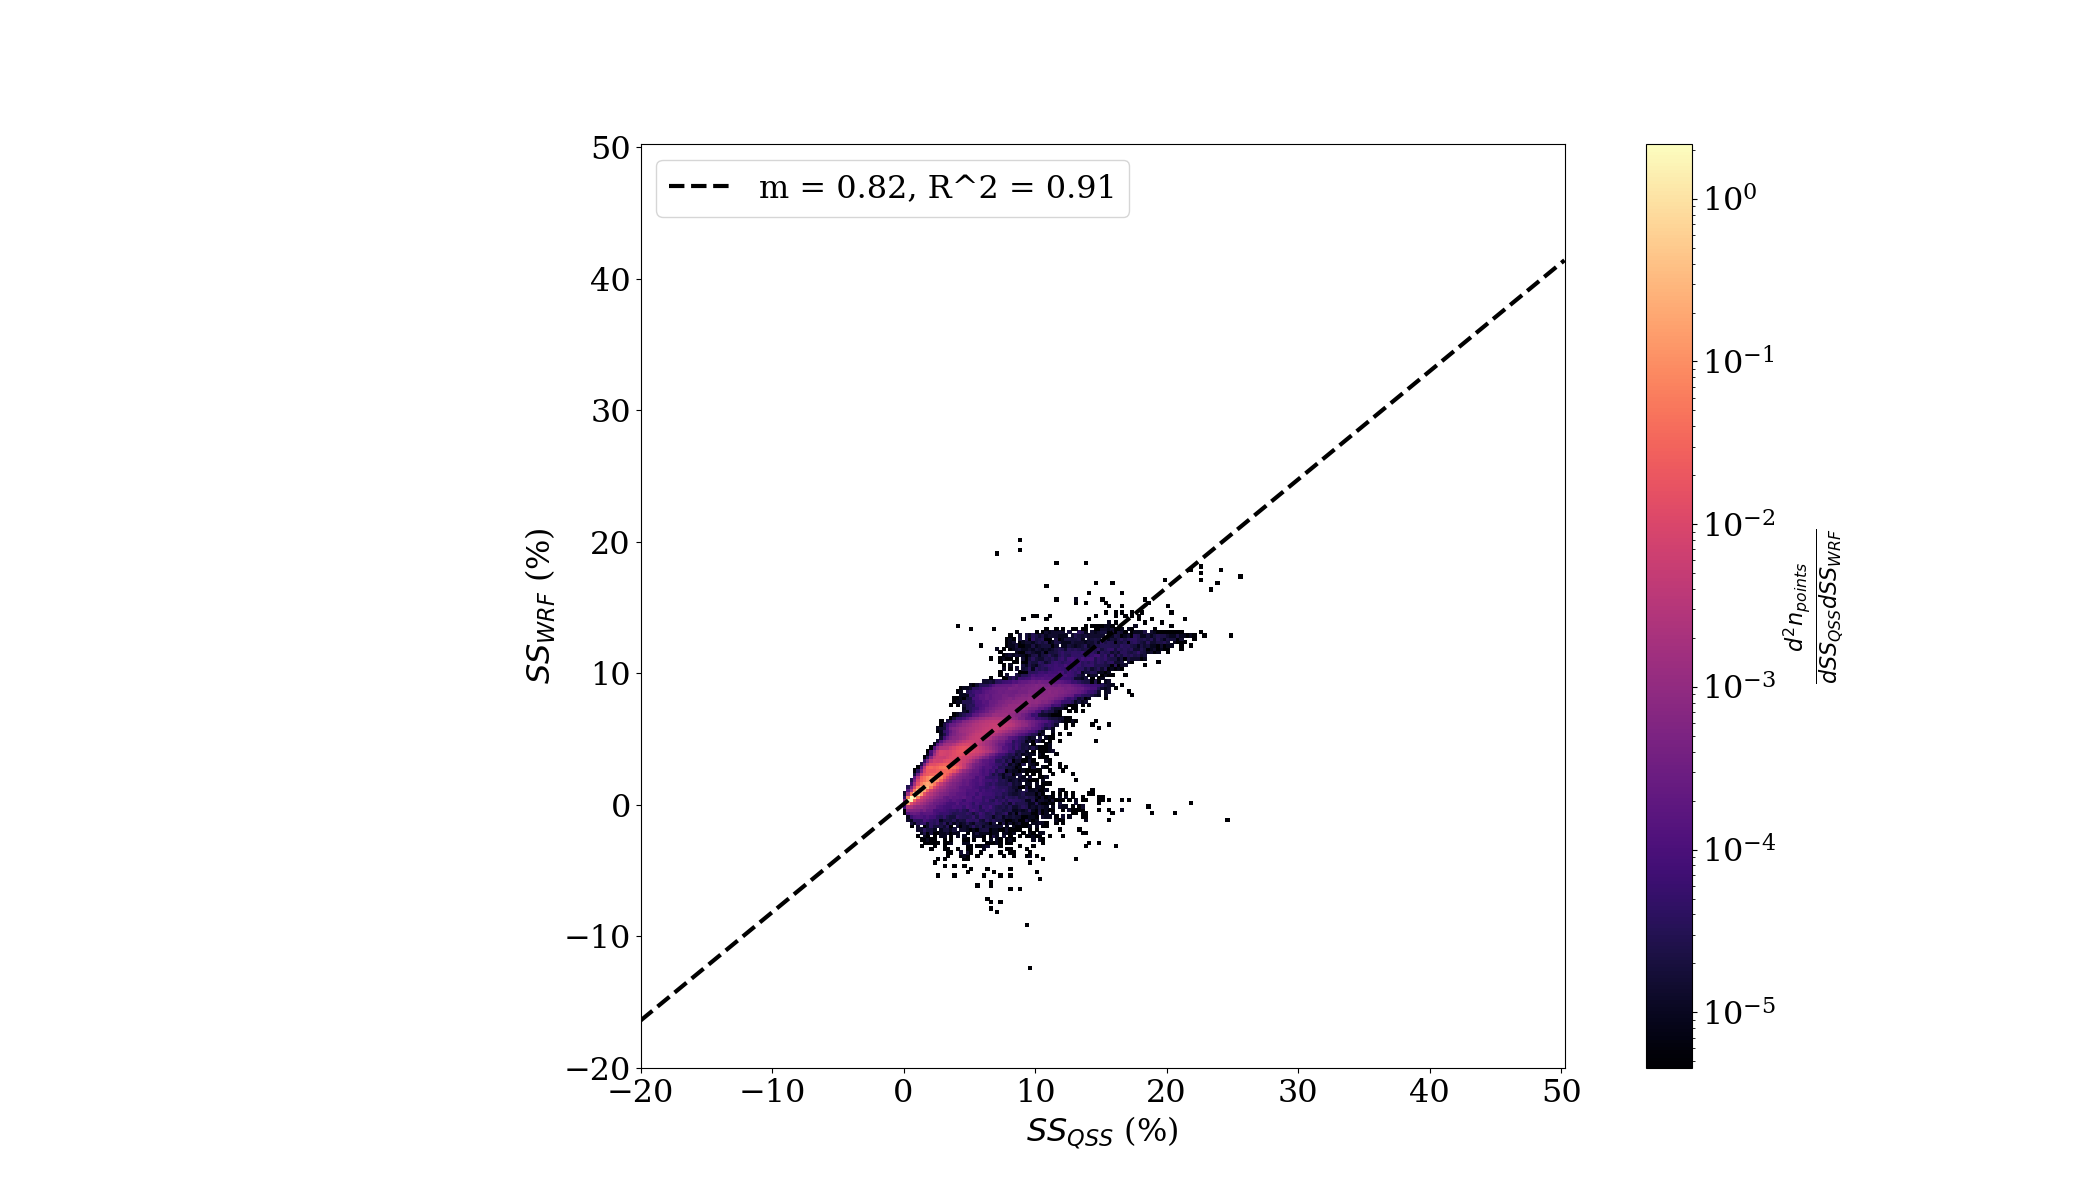
\includegraphics[width=\textwidth]{revmywrf/v1_FINAL_heatmap_ss_qss_vs_ss_wrf_Polluted_figure.png}
		\caption{Polluted case.}
		\label{wrfvsqsspoll}
	\end{subfigure}
	\caption{Actual ($SS_{WRF}$) vs predicted ($SS_{QSS}$) supersaturation. Color indicates density of data points; note the scale is logarithmic.}
	\label{wrfvsqss}
\end{figure}

Because we use slightly different filtering criteria than that employed in Fan et al to examine updrafts, we first verify that our selected cloudy updraft points yield similar SS profiles in the WRF simulation as those found in the latter work. In Figure \ref{wrfbipanel} we plot vertical SS profiles for all cloudy updraft points as well as the upper 10th percentile with respect to vertical wind velocity. In \cite{Fan2018} they consider a restricted subdomain around the T3 field station, indicated in Figure S8 of the supplementary information for that paper; we do not see a major qualitative difference when including this additional criterion; see Figure \ref{wrfsubdombipanel}. We do indeed find the high SS values reported by Fan et al (maximum values of 13\% in both polluted and unpolluted cases from the upper 10th percentile dataset), confirming that our filtering criteria establish a fair basis for comparison here. Note however that, in the righthand panels of Figure \ref{wrfbipanel}, the vast majority of cloudy updraft points are found at altitudes with relatively low average SS.

\begin{figure}[ht]
	\centering
	\begin{subfigure}{0.7\textwidth}
		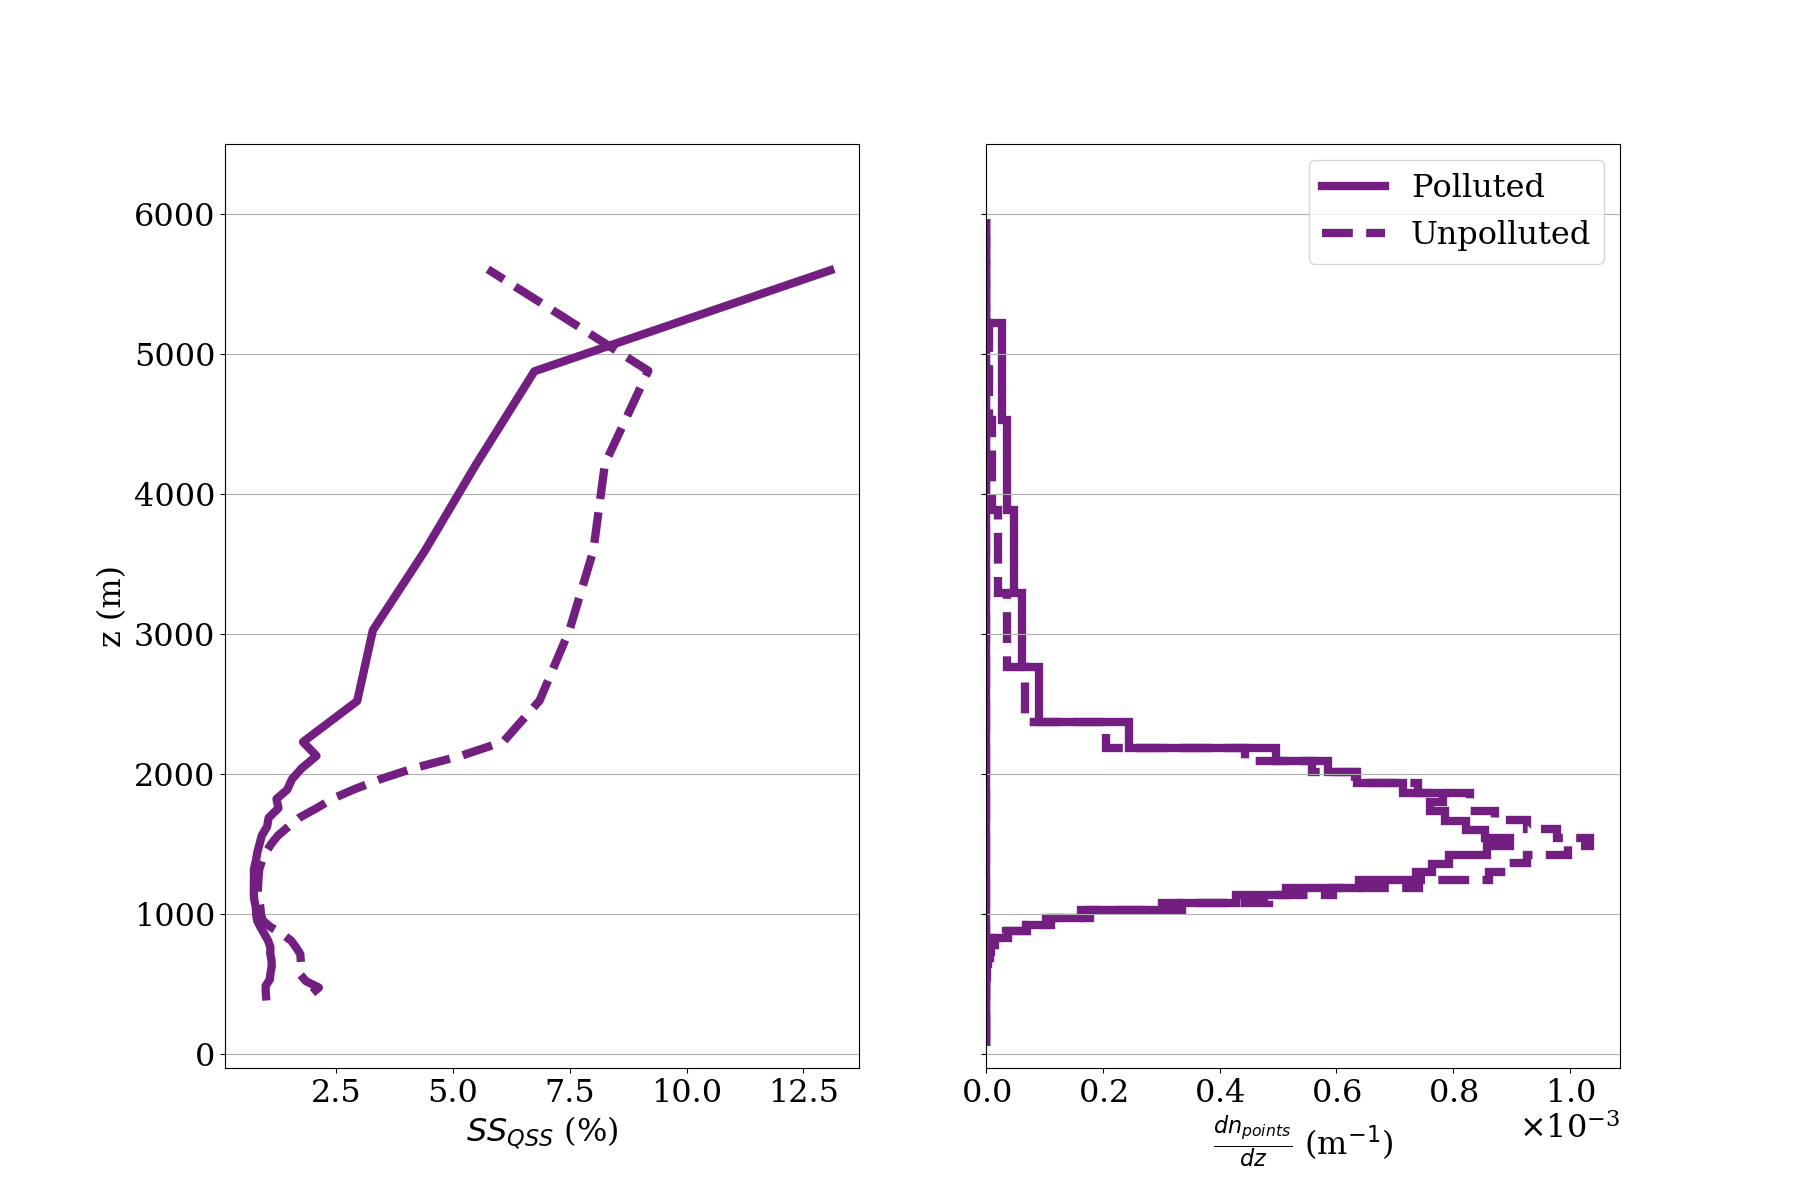
\includegraphics[width=\textwidth]{revmywrf/v5_FINAL_bipanel_ss_qss_vs_z_allpts_figure.png}
		\caption{}
		\label{wrfbipanelallpts}
	\end{subfigure}
	\begin{subfigure}{0.7\textwidth}
		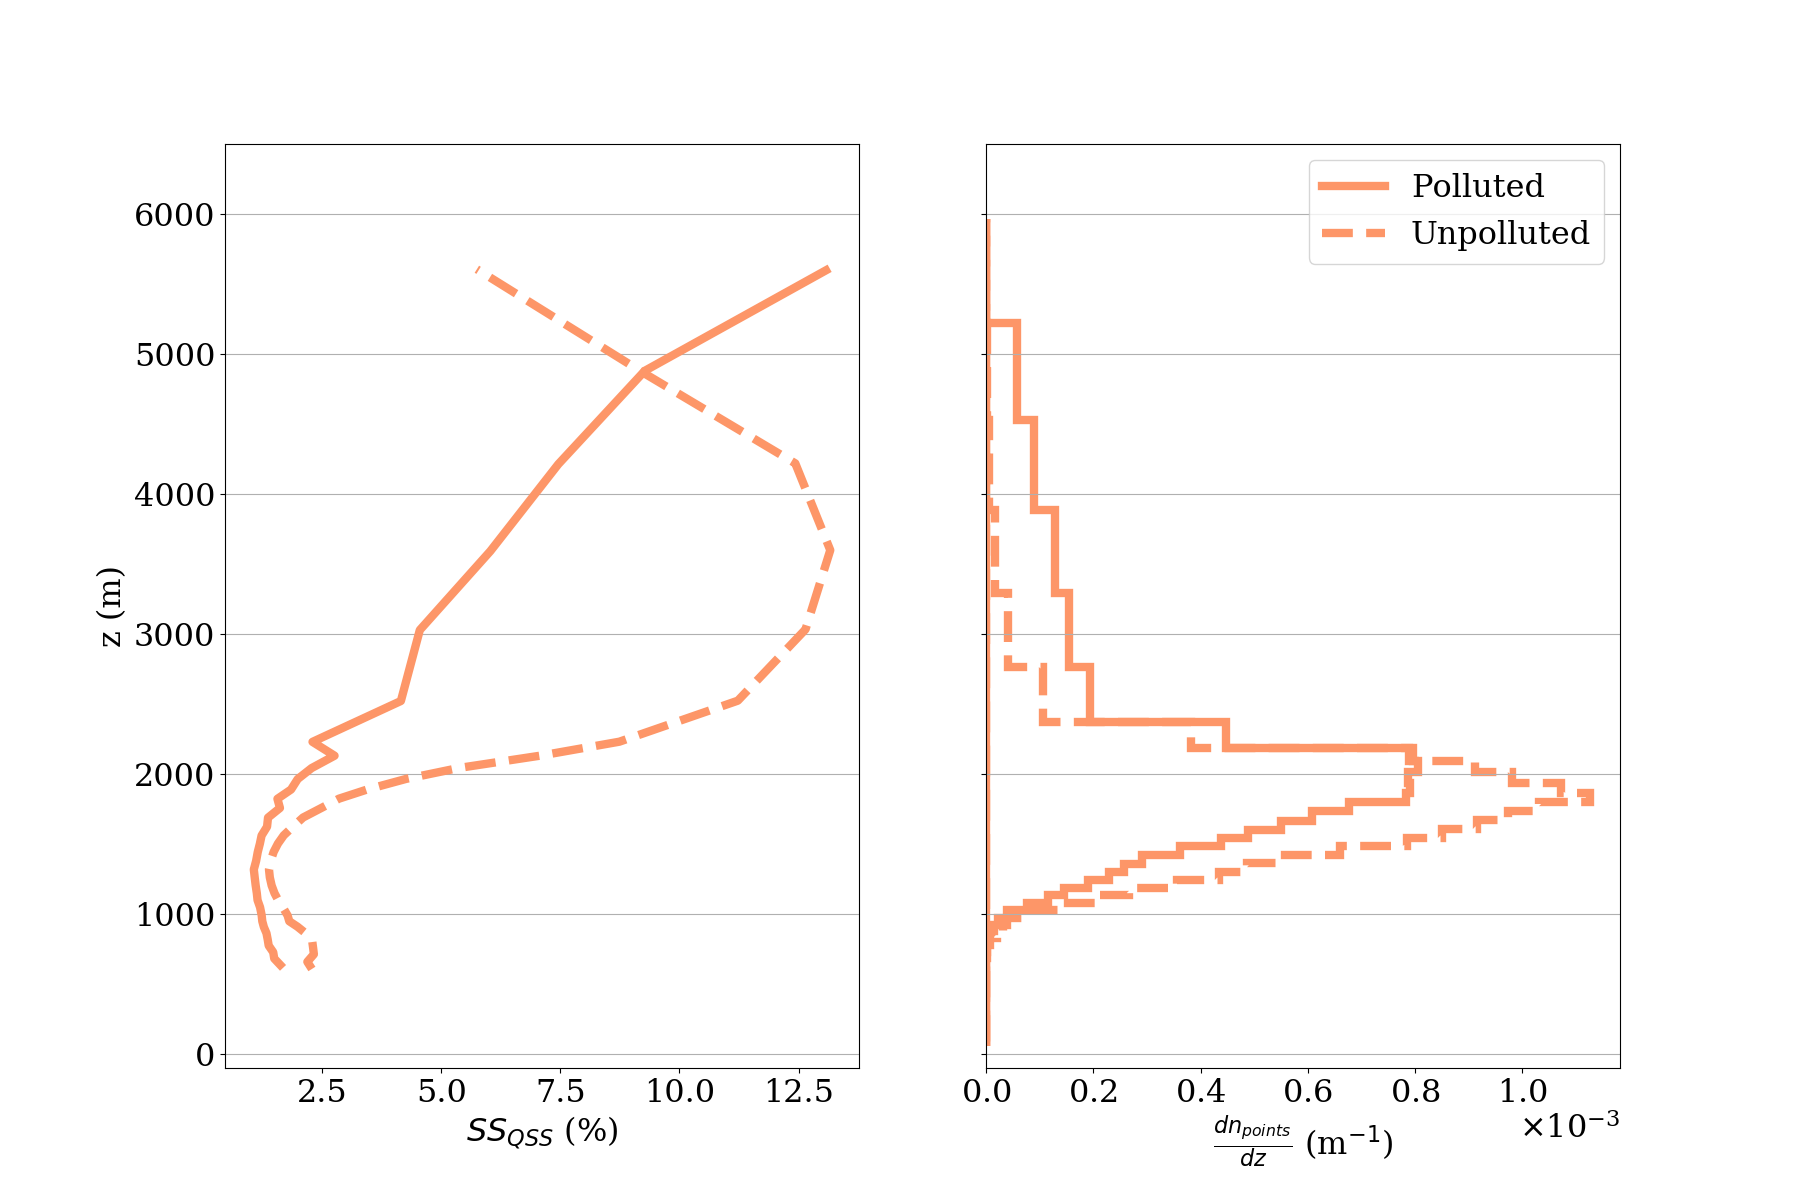
\includegraphics[width=\textwidth]{revmywrf/v5_FINAL_bipanel_ss_qss_vs_z_up10perc_figure.png}
		\caption{}
		\label{wrfbipanelup50perc}
	\end{subfigure}
	\caption{SS profiles (left) and number density of sampled points (right) for a) all cloudy updraft points; b) top 10\% of cloudy updraft points with respect to vertical wind velocity, in WRF simulation conducted by Fan et al. Each point in the vertical profile represents an average over all times and horizontal coordinates for a given vertical grid coordinate.}
	\label{wrfbipanel}
\end{figure}

\clearpage
\newpage

We now seek to determine whether such high values actually occur in nature. First we look at data from the HALO flights in September and October of 2014 (see Methods/SI for details on selection of dates for this analysis) [ \klcomm{how to cite?} ]. Figure \ref{halobipanel} shows the analogue of Figure \ref{wrfbipanel} using data from all HALO flight dates combined. We find no points with average SS above 1 \%, even when limiting to the strongest updrafts in the combined dataset.

\begin{figure}[ht]
    \centering
    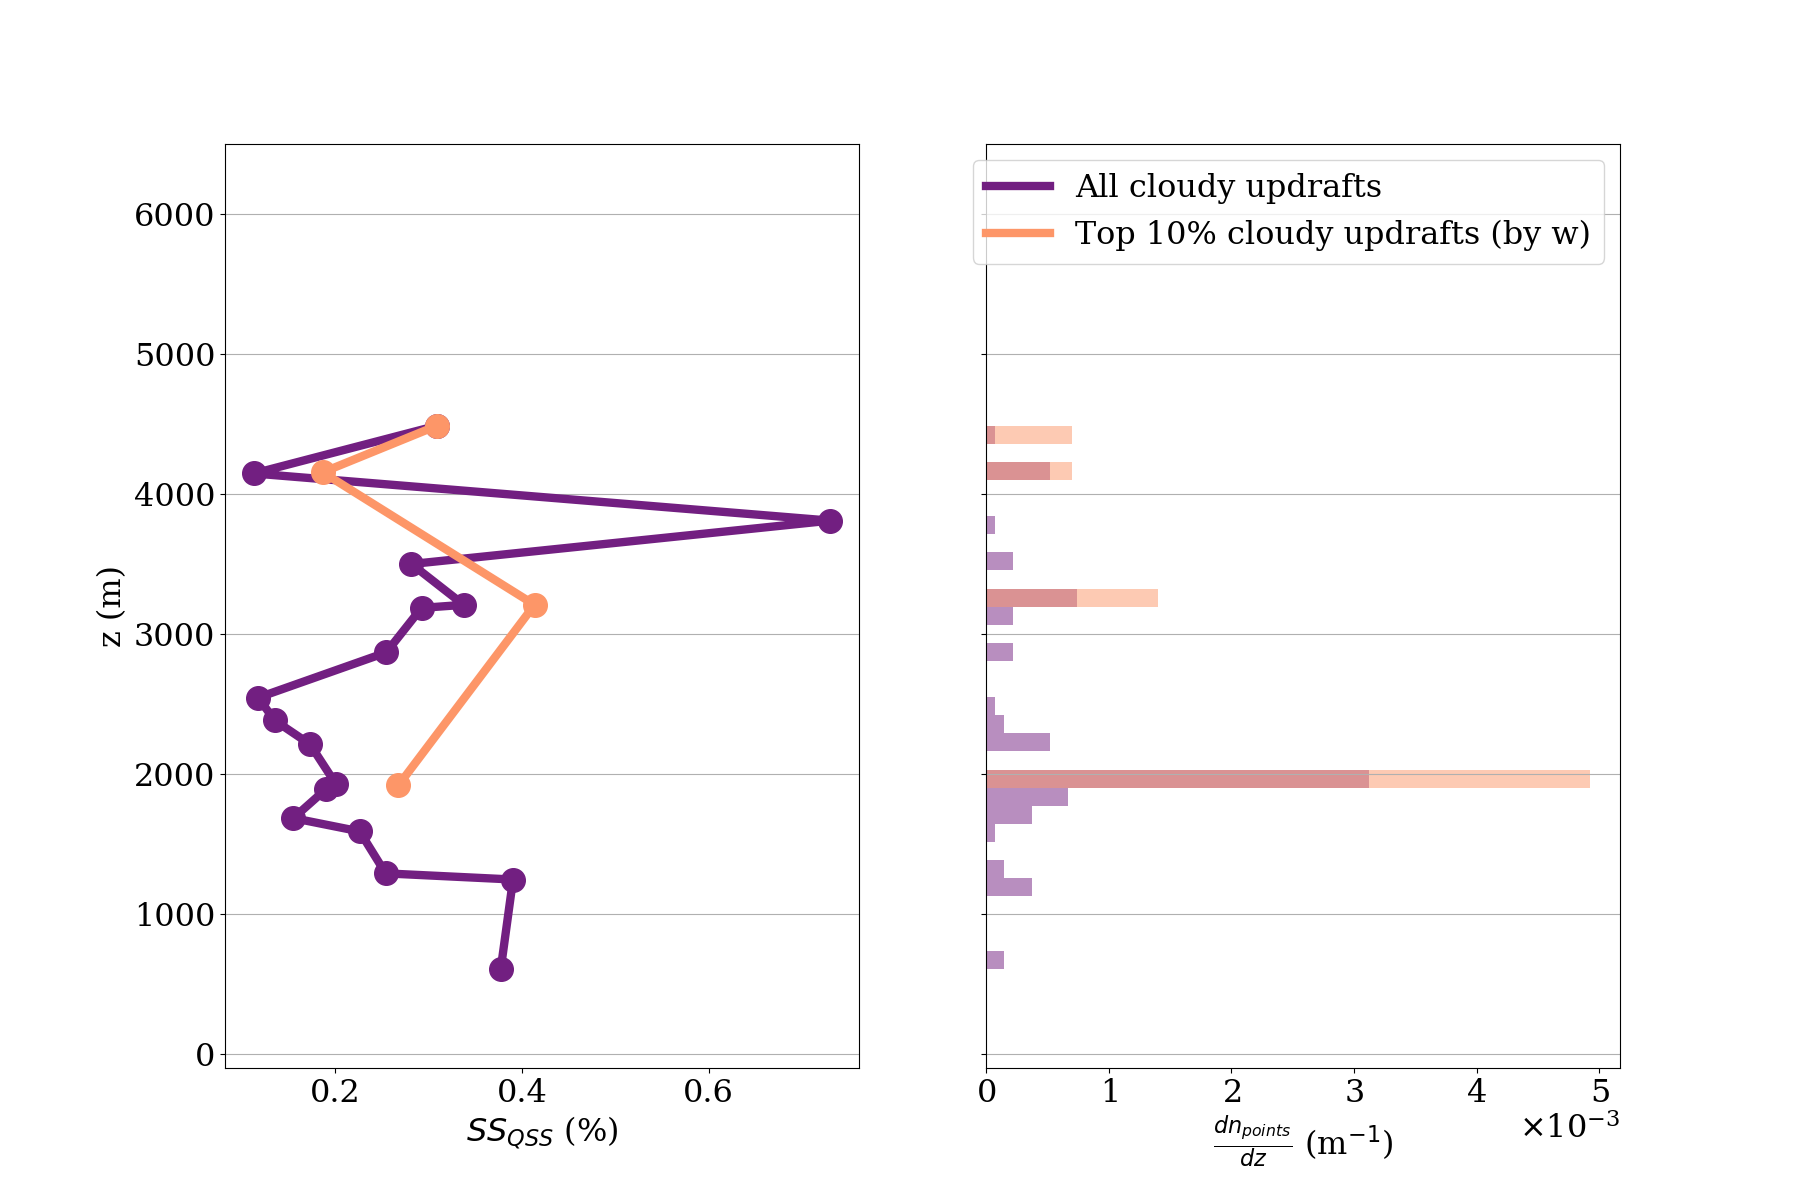
\includegraphics[width=9cm]{revhalo/v3_FINAL_combined_bipanel_ss_qss_vs_z_figure.png}
    \caption{SS profiles (left) and number density of sampled points (right) from HALO flight campaign (all dates combined). Each point in the vertical profile represents an average over all times and horizontal coordinates for a given vertical interval (equally-spaced). SS profile is plotted with markers so as not to obscure intervals with missing data.}
    \label{halobipanel}
\end{figure}

Finally, we examine a second experimental dataset from the first phase of the CAIPEEX campaign \cite{Kulkarni2012}. Although no UAP$_{<50}$ concentration measurements are available during this phase of the experiment, measurements of aerosols with diameters in the range of 0.1-3 $\mu$m showed total aerosol concentrations ranging from 700/ccm to 2500/ccm in the BL (see Figure 3(b) in \cite{Prabha2011} and Figure 4(a) in \cite{Kulkarni2012}). Reliable rain drop particle size distributions are unavailable from the flight dates in this analysis phase of the experiment, but we observe that exclusion of raindrops from the calculation of QSS SS leads to a systematic overestimation of the true SS (see Methods/SI). Therefore we take the SS profiles in Figure \ref{caipeexbipanel} as an upper bound. We observe slightly higher values relative to those from the HALO flights, although we still don't find such high values as those output by the WRF models for the middle troposphere.


\begin{figure}[ht]
    \centering
    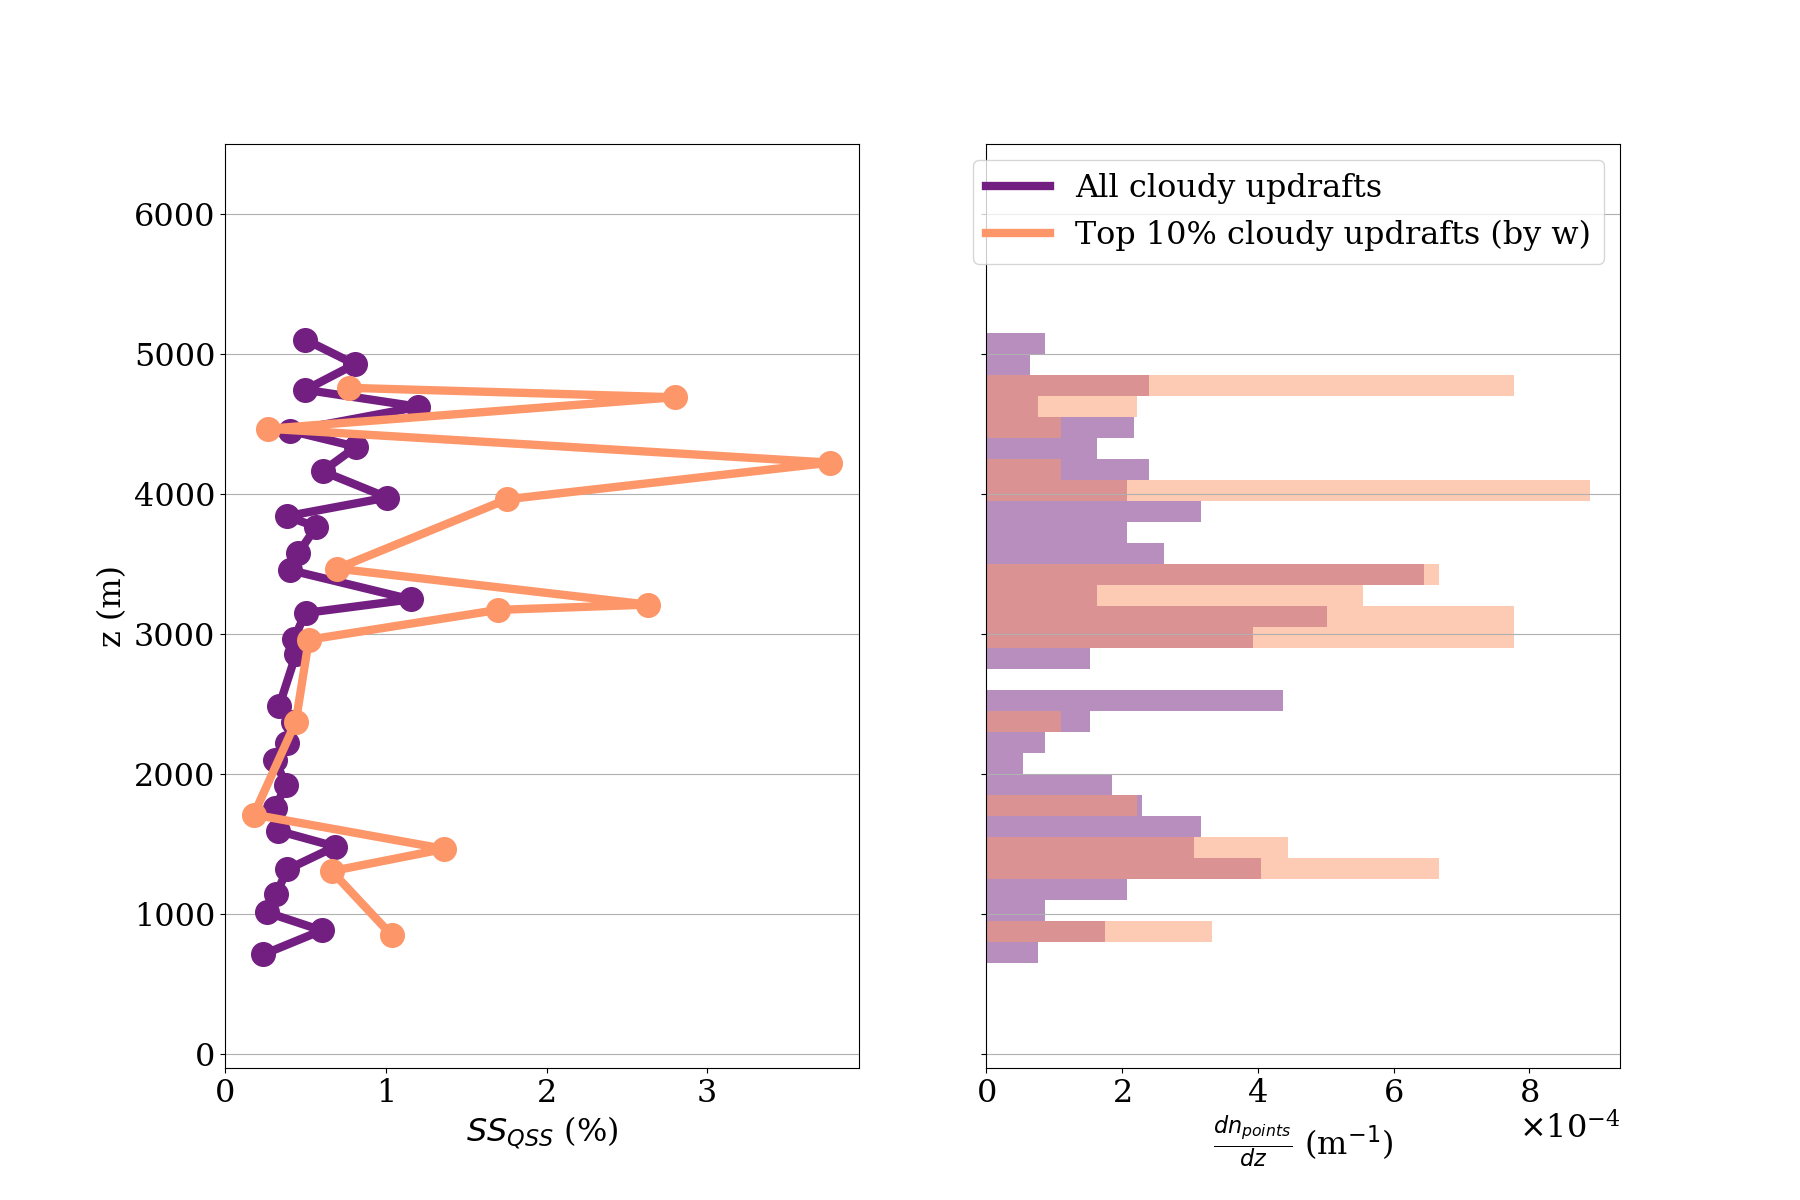
\includegraphics[width=9cm]{revcaipeex/v3_FINAL_combined_bipanel_ss_qss_vs_z_figure.png}
    \caption{SS profiles (left) and number density of sampled points (right) from CAIPEEX flight campaign (all dates combined). Each point in the vertical profile represents an average over all times and horizontal coordinates for a given vertical interval (equally-spaced). SS profile is plotted with markers so as not to obscure intervals with missing data. See text for comments on the dataset.}
    \label{caipeexbipanel}
\end{figure}

We can use Equation \ref{dT} and the SS profiles in Figures \ref{wrfbipanel}-\ref{caipeexbipanel} to infer a buoyancy profile for a hypothetical non-supersaturated parcel. For this analysis we take the temperature of the parcel equal to that of the environment (i.e., what has been measured). The resulting error in the value of $\delta T$ in Equation \ref{} is quadratic in $\delta RH$, which is acceptable for our purposes. In Figure \ref{dTprofiles} we plot $\delta T$ profiles from both WRF simulations and field campaigns side-by-side. We use these profiles to derive enhancements in $CAPE$ for the non-supersaturated parcel as:
\begin{equation}
\label{dCAPE}
\delta CAPE = g \int dz \frac{\delta T}{T}
\end{equation}
where we again approximate $T$ as the environmental temperature and integrate from 647 to 4488 m, the common vertical domain for all four curves in Figure \ref{dTprofiles}. We find values of $\delta CAPE$ of 4, 6, 36, and 68 J/kg for HALO, CAIPEEX, WRF (polluted), and WRF (unpolluted), respectively. Neglecting any other physical energy sinks as above, these translate to vertical velocity enhancements of about 3 m/s in the field campaigns and 10 m/s in the simulations.

\begin{figure}[ht]
    \centering
    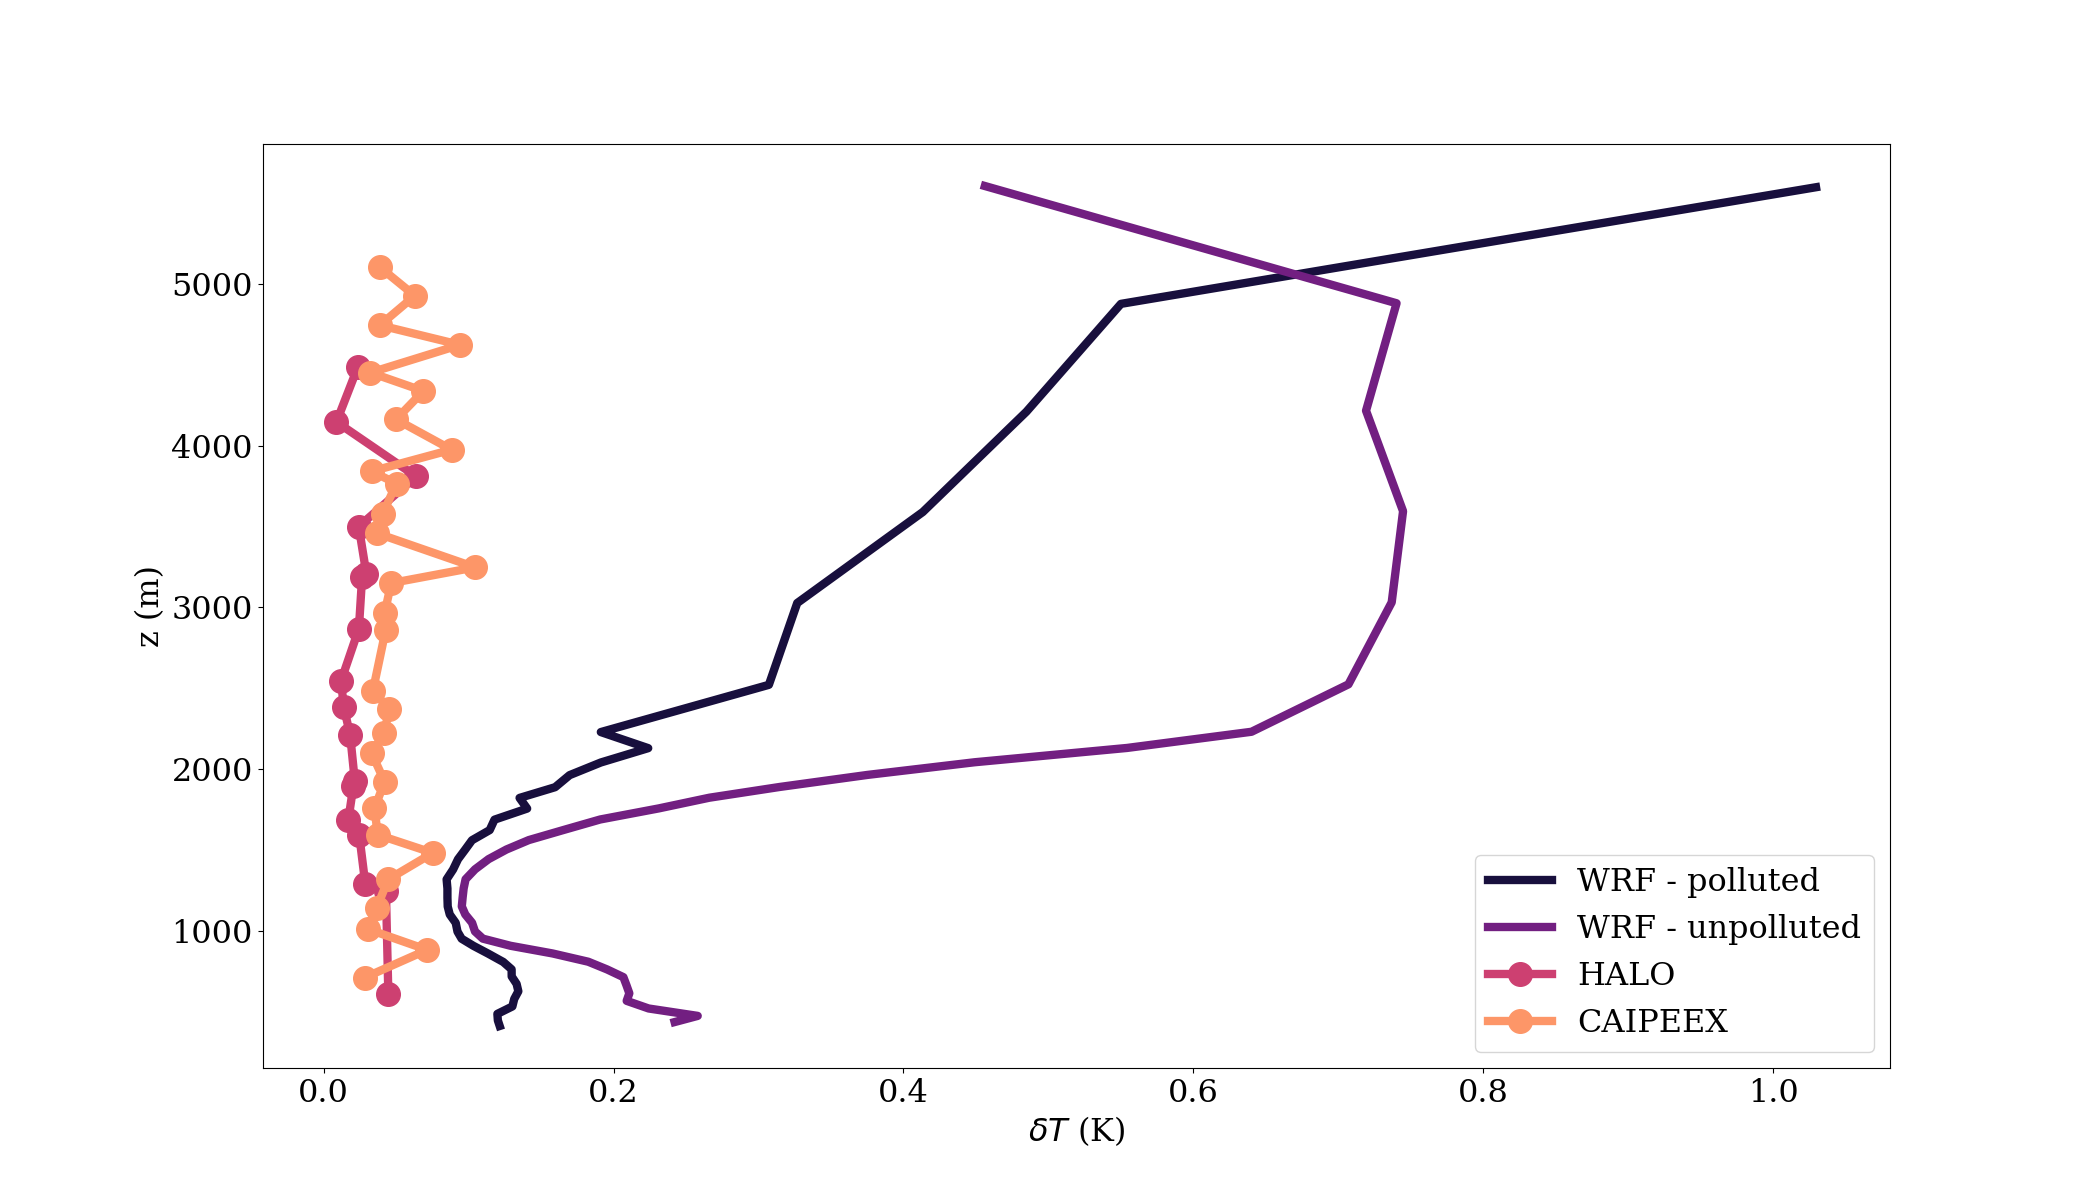
\includegraphics[width=12cm]{revmywrf/v1_FINAL_combined_dT_profile_figure.png}
    \caption{Profiles for $\delta T$ of a non-supersaturated ($RH=1$) parcel ascending in an environment with SS profiles shown in Figures \ref{wrfbipanel}-\ref{caipeexbipanel}, using Equation \ref{dCAPE}. SS profiles for HALO and CAIPEEX are plotted with markers so as not to obscure intervals with missing data.}
    \label{dTprofiles}
\end{figure}

One possible counterargument is that the aerosol concentrations in the BL during the dates of the HALO flights might have been significantly higher than those during the dates considered in Fan's paper, thus precluding the occurence of high SS values in the troposphere. In order to investigate this, we use the aerosol particle size distribution measured by the scanning mobility particle sizer (SMPS) in Manacapuru, located southwest of Manaus (PI: Chongai Kuang). This intrument measures particle concentrations in the diameter range 11.1-469.8nm. In Figure \ref{goamahist}, we show that, while we do indeed see higher total aerosol concentrations on average during the HALO flight date range (3500/ccm vs 2400/ccm), the UAP50 concentration is on average lower (670/ccm vs 1600/ccm). In fact, the aerosol concentrations used in the WRF simulations are much lower than those observed during the day the simulation takes place, which is not justified quantitatively in that study.

We note additionally that the positive experimental correlation between concentration of UAP50 and maximum vertical velocity during the dates studied by Fan et al is not significant even at the 90\% confidence level - the least-squares slope parameter for their data set (the plot of which we reproduce in Figure \ref{fans2a}) has a p-value of 0.11.
\begin{figure}[ht]
	\centering
	\begin{subfigure}{0.7\textwidth}
		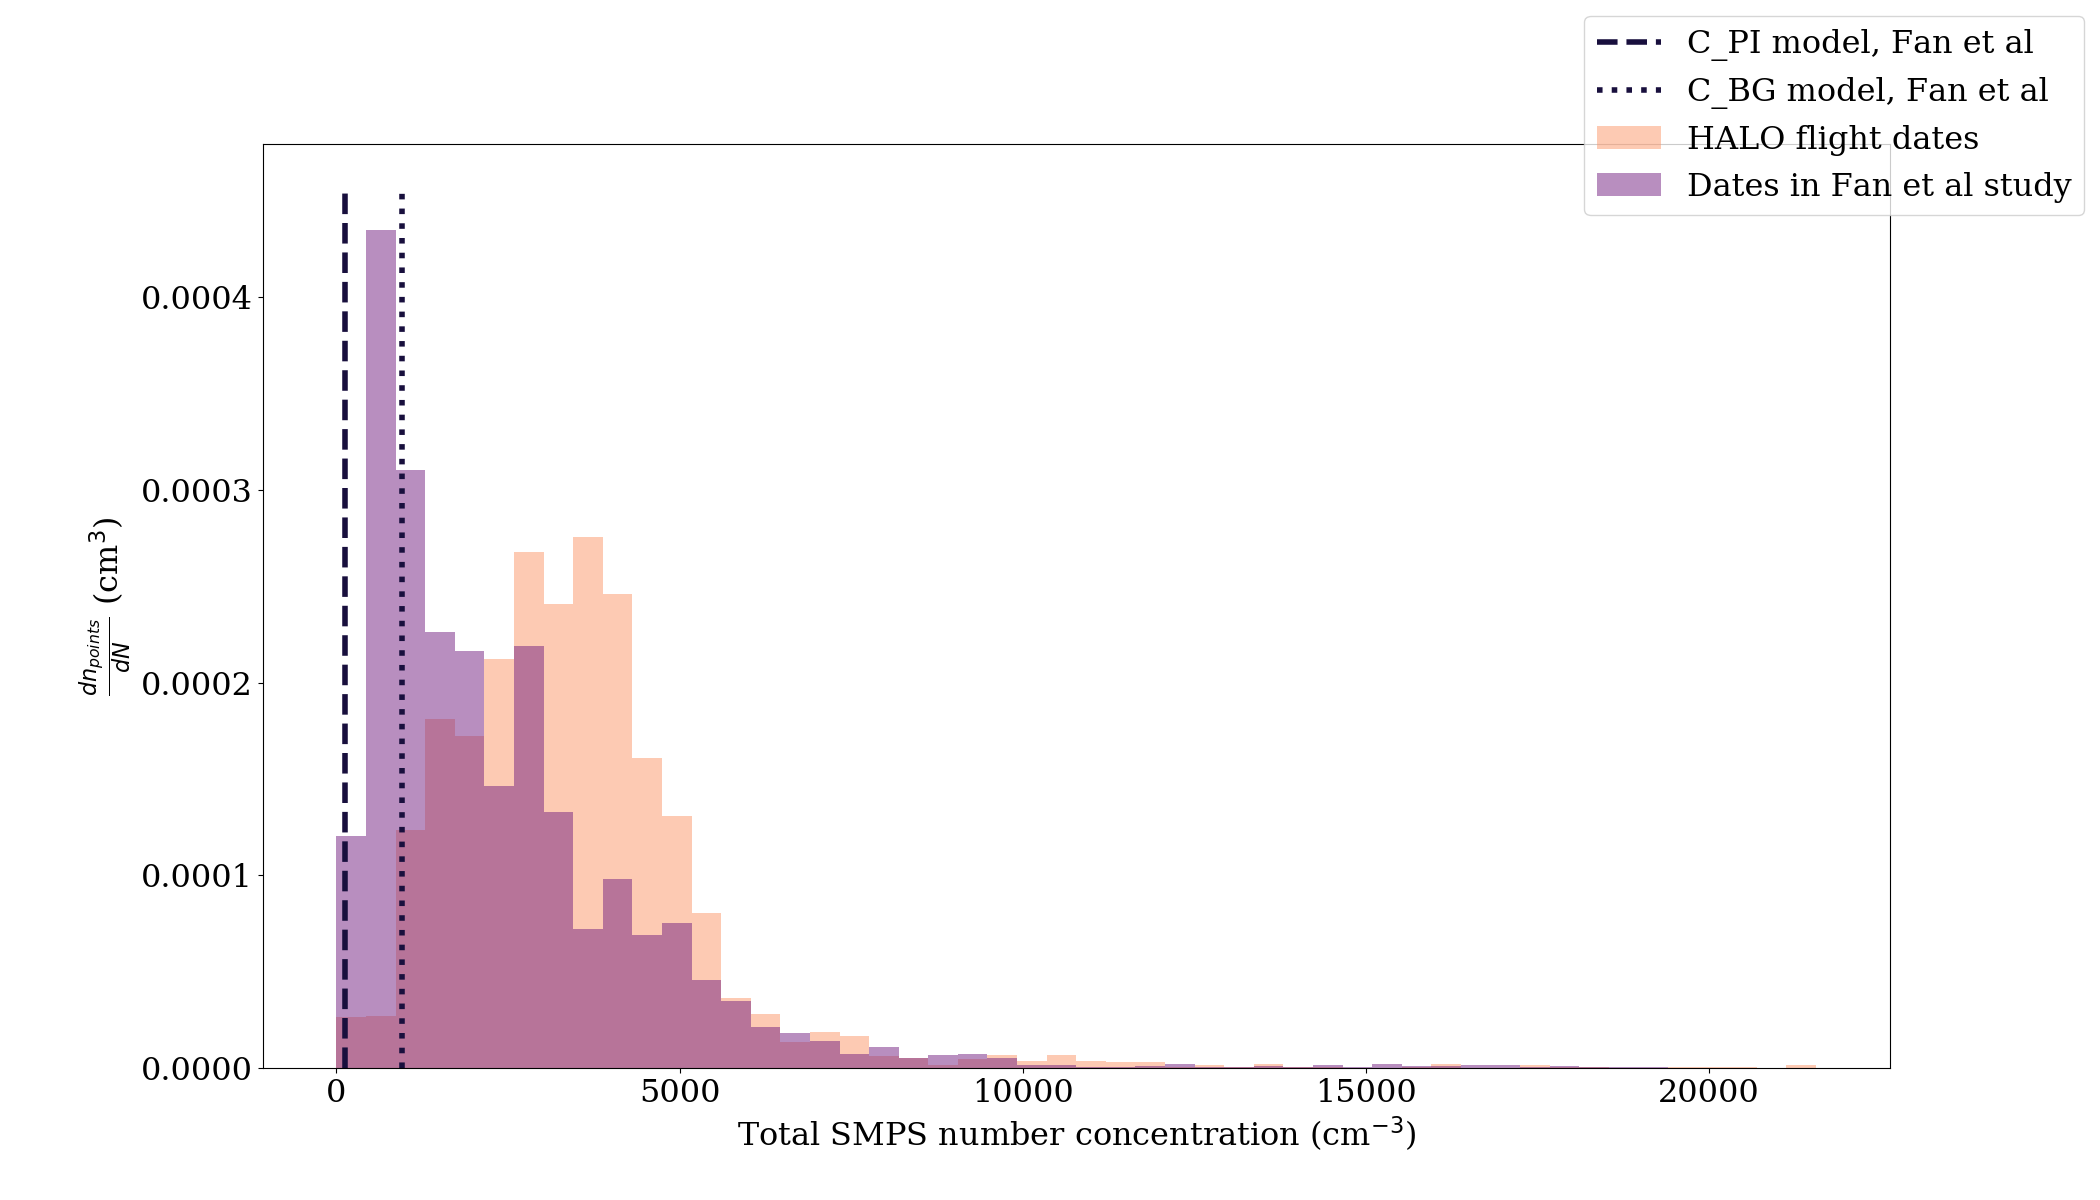
\includegraphics[width=\textwidth]{goama/v1_FINAL_tot_compare_nconc_hist_alldates_figure.png}
		\label{goamatothist}
		\caption{}
	\end{subfigure}
	\begin{subfigure}{0.7\textwidth}
		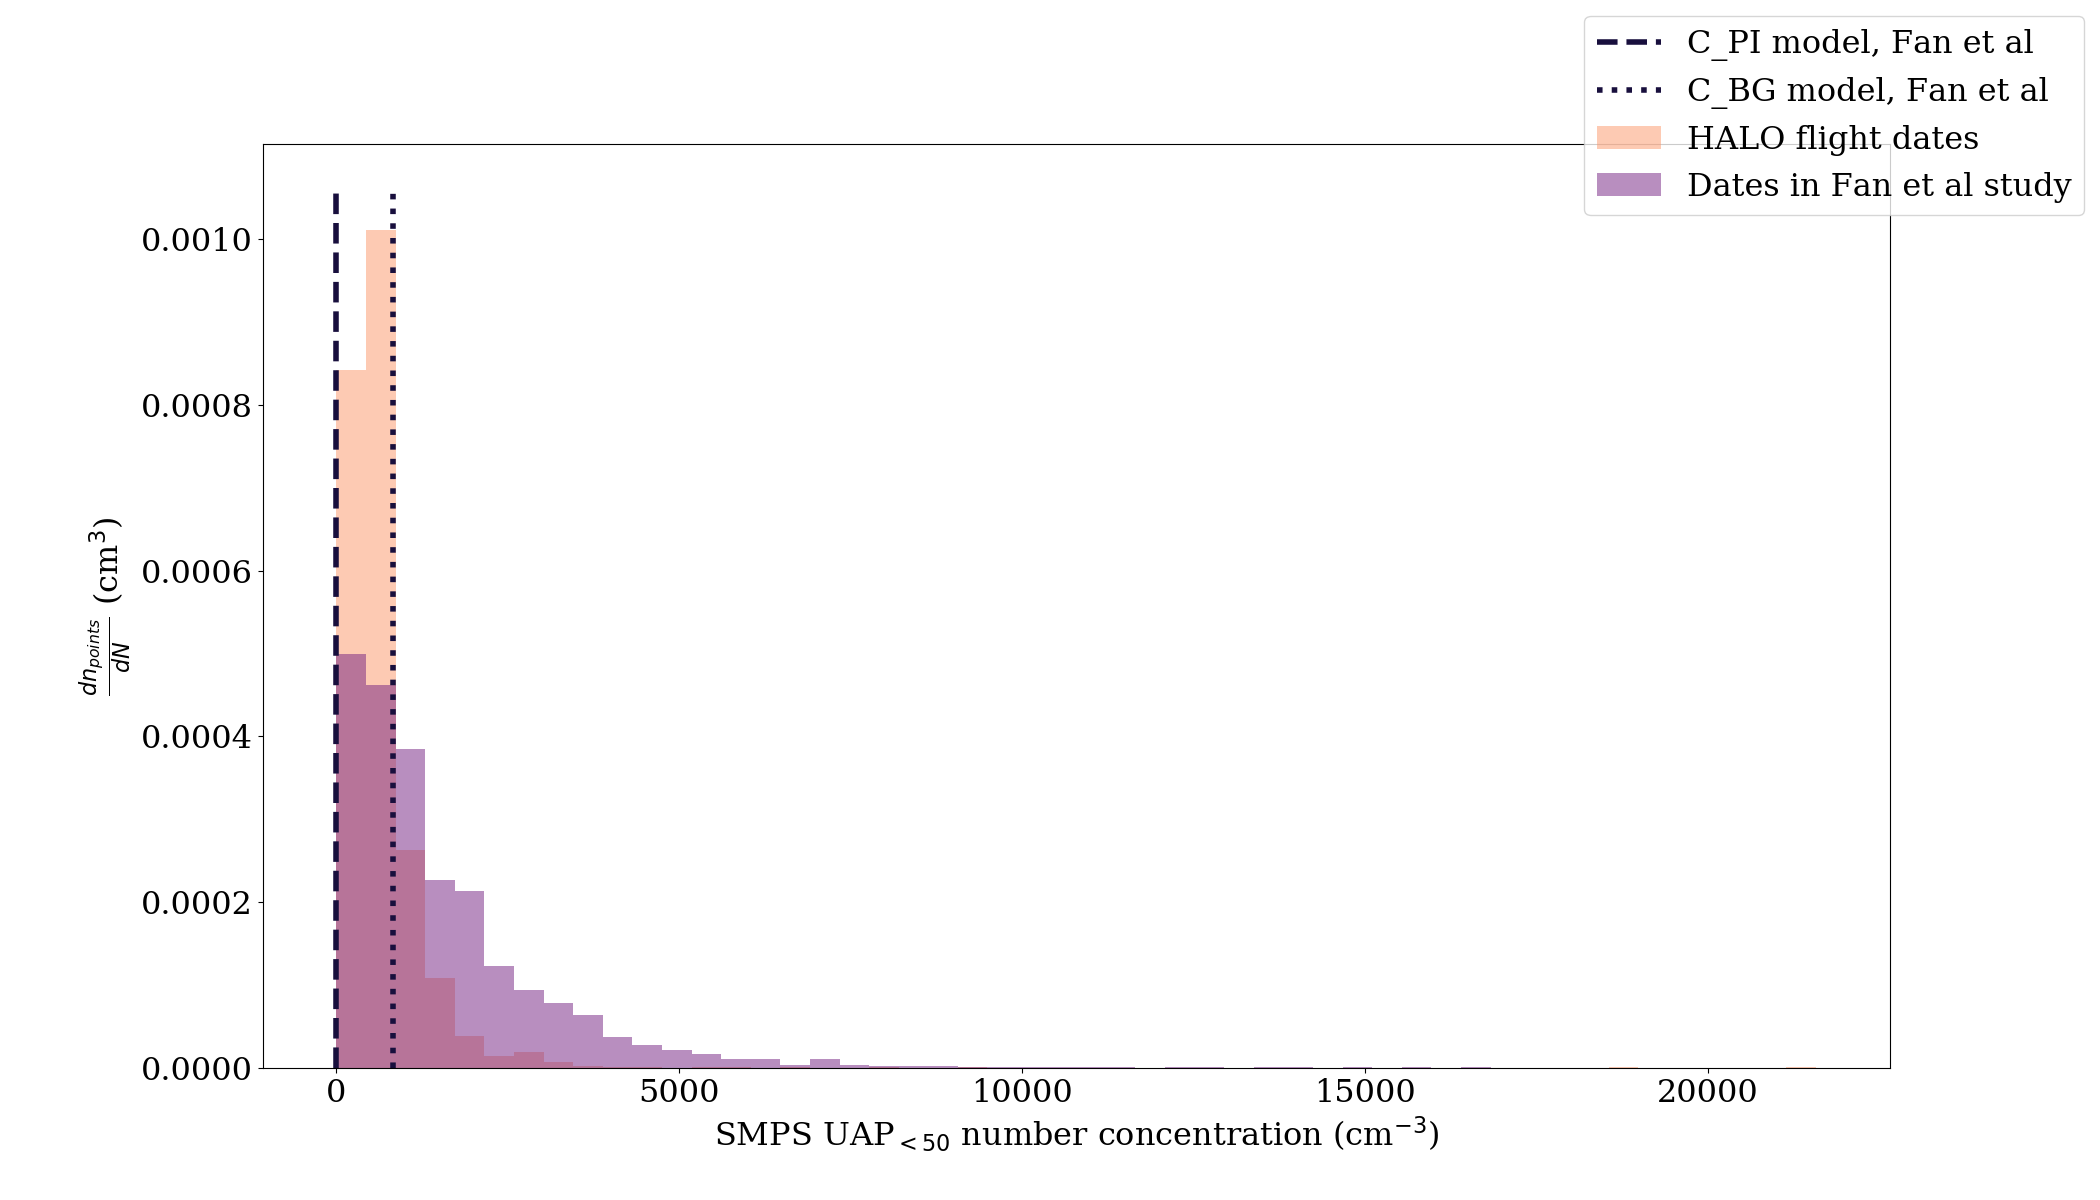
\includegraphics[width=\textwidth]{goama/v1_FINAL_uap50_compare_nconc_hist_alldates_figure.png}
		\label{goamauap50hist}
		\caption{}
	\end{subfigure}
	\caption{Distribution of aerosol concentration measurements by the ground-based SMPS at Manacapuru, Brazil; a) entire size range, b) only particles with diameter greater less than 50nm. HALO flight dates are the same as those represented in Figure \ref{halobipanel} (see Methods/SI for details). Dashed (dotted) lines show initial concentrations in the BL of the WRF simulation of polluted (unpolluted) conditions.}
	\label{goamahist}
\end{figure}
\begin{figure}[ht]
    \centering
    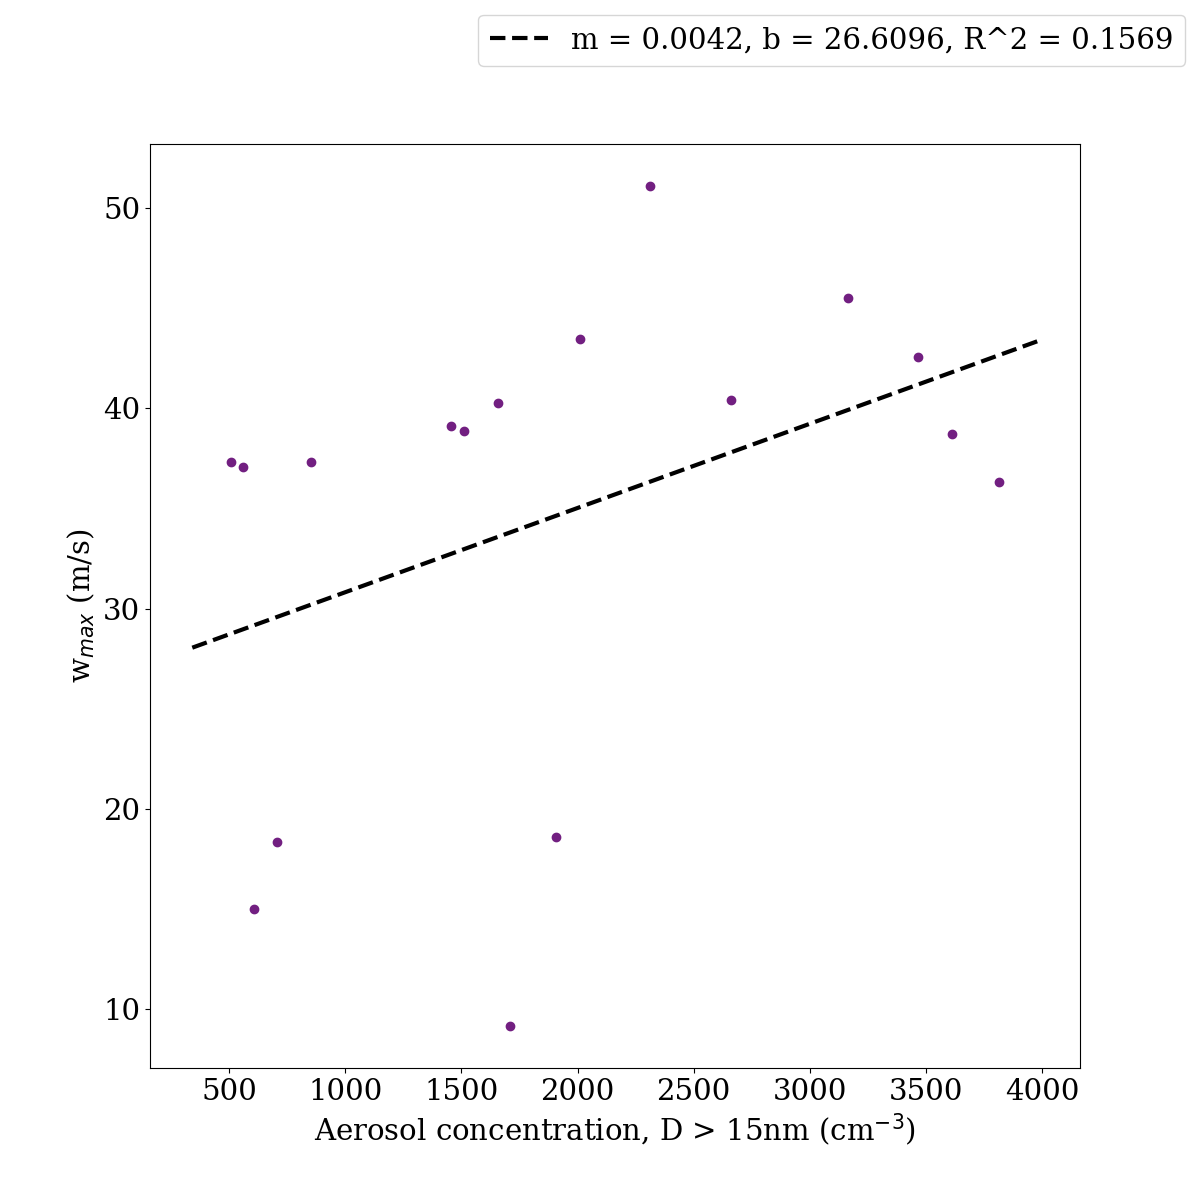
\includegraphics[width=12cm]{revhalo/v1_FINAL_fan_fig_s2a.png}
    \caption{Ground-based total (including UAP50) aerosol concentration measurements versus maximum vertical wind velocity in convective cores; reproduced from Figure S2(a) of \cite{Fan2018}.}
    \label{fans2a}
\end{figure}

Another possible counterargument is that the flight campaigns simply didn't fly through strong enough updrafts. However the vertical velocity distributions from the campaigns are quite similar to that from the simulations. See Figure \ref{combinedwhist}. 

\begin{figure}[ht]
    \centering
    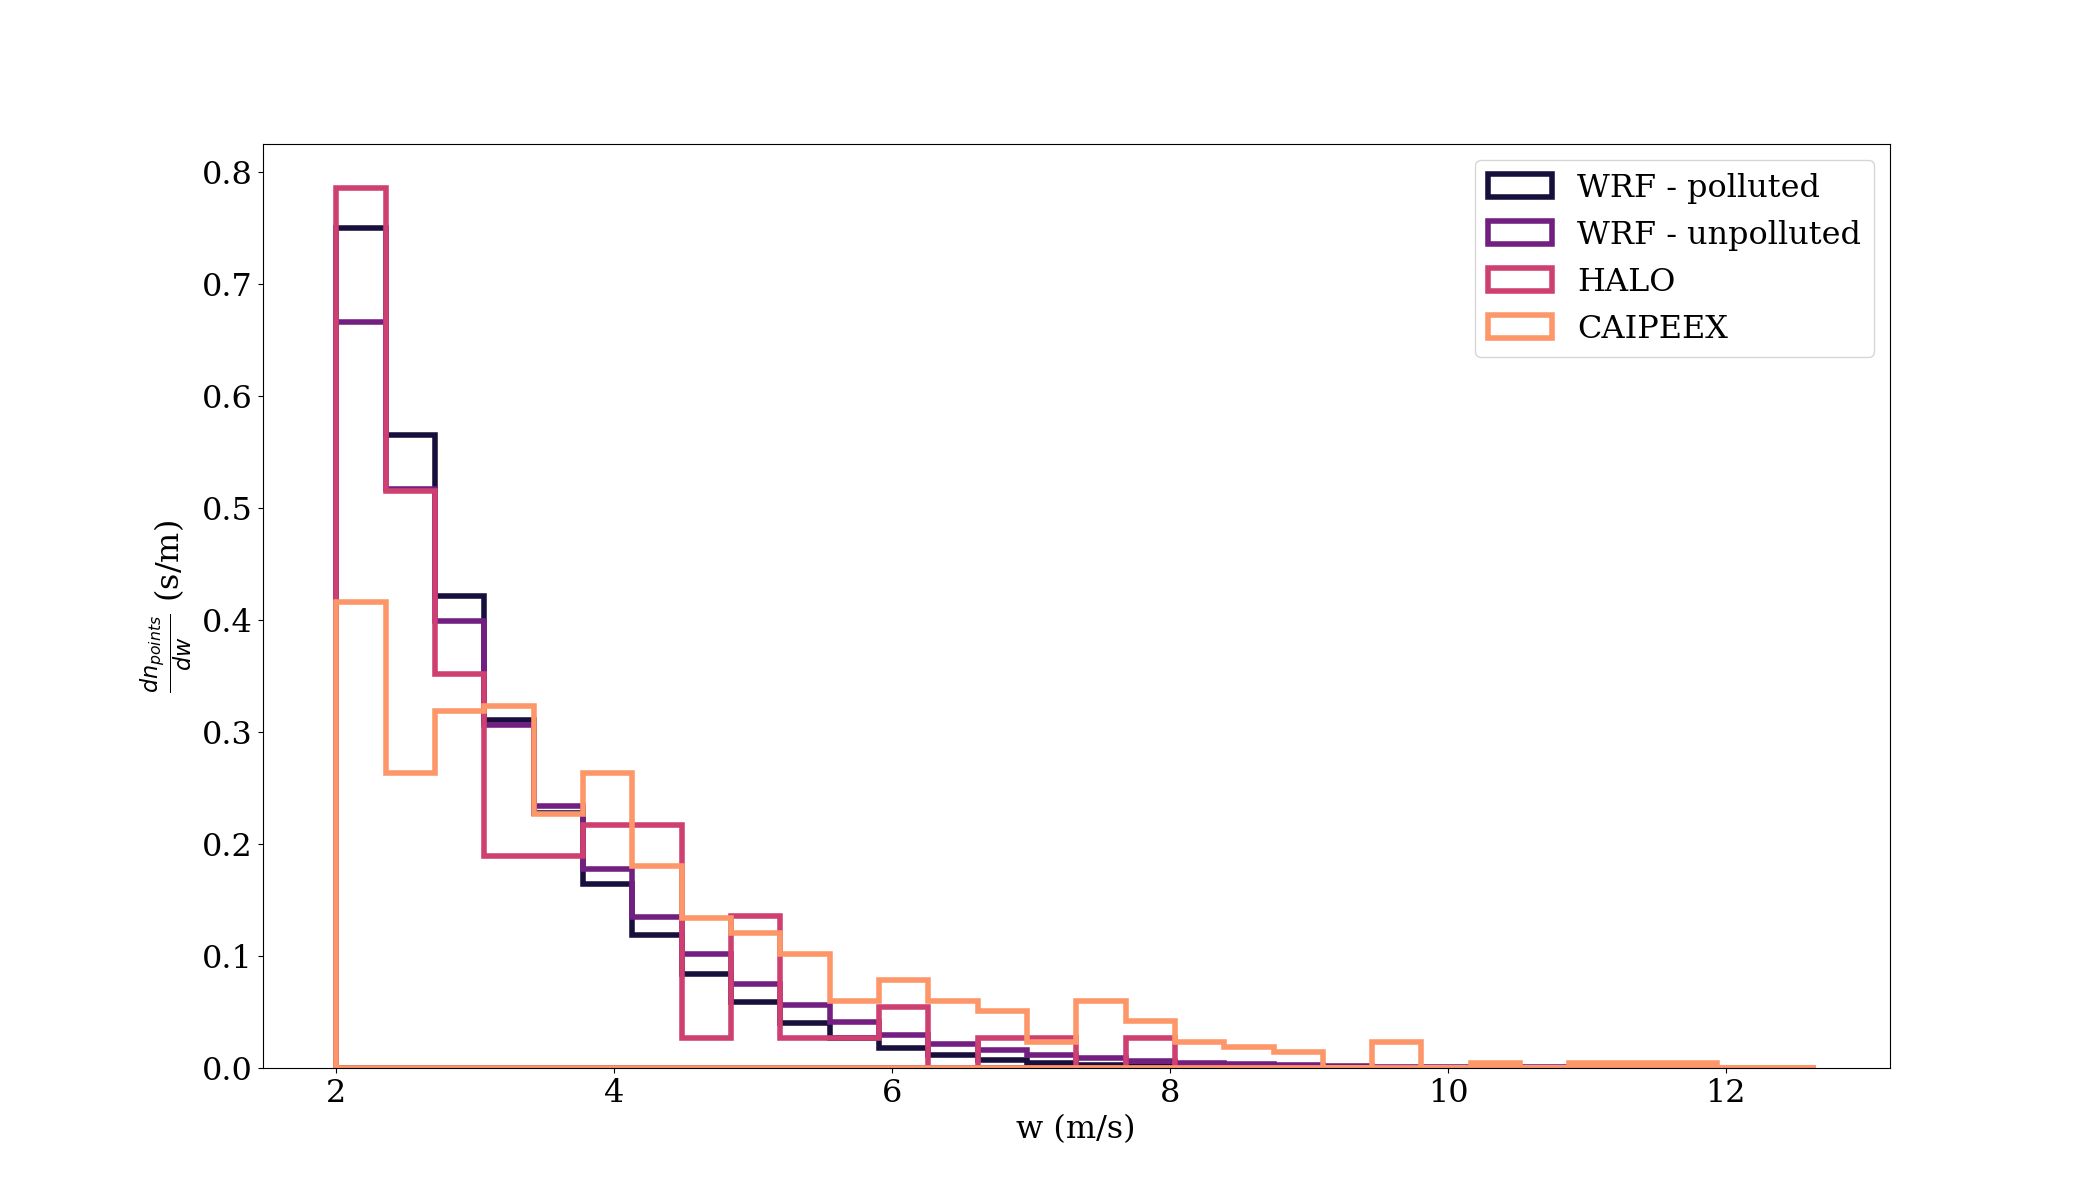
\includegraphics[width=12cm]{revmywrf/v2_FINAL_combined_w_hist_figure.png}
    \caption{Vertical wind velocity distribution from simulations and field campaigns. Using filtering criteria outlined in the text.}
    \label{combinedwhist}
\end{figure}

Conclusion: The WPIM as proposed by Fan et al requires the average temperature profile of the troposphere to be set by relatively clean (high-SS) convection, in order for more polluted (low-SS) convection to experience an enhancement in buoyancy. However, we find no evidence that the high SS values reported by Fan's model actually occur in nature, which weakens the possibility of measureable invigoration effects - in particular, we estimate an upper bound on vertical velocity enhancement of $\approx$ 3 m/s from the HALO and CAIPEEX flight campaigns, compared to $\approx$ 10 m/s from Fan's control simulations in WRF. The relatively low aerosol concentrations used to initialize the simulations, in combination with possible irregularities in microphysical parameterizations, may be to blame for the anomalously high SS values in the WRF output.

\clearpage
\newpage

\section{Methods/SI}

\subsection{WRF}

Model output for control simulations of polluted (``C\_BG") and unpolluted (``C\_PI") scenarios were provided by Fan et al; see that paper and accompanying SI for detailed explanations of model parameters and initializations.

In this paper, we use the following form of the QSS SS equation after \cite{Rogers1989} (with $SS_{QSS}$ given as a percentage):
\begin{equation}
\label{fullss}
SS_{QSS} = \frac{A(T) w}{4\pi B(\rho_a, T) \langle f(r)\cdot r\rangle n}*100,
\end{equation}
where:
\begin{align}
A(T) &= \frac{g}{R_a T}\Big(\frac{L_v R_a}{C_{ap} R_v T} - 1\Big)\big(F_d(T) + F_k(T)\big)\nonumber\\
F_d(T) &= \frac{\rho_w R_v T}{D e_s(T)}\nonumber\\
F_k(T) &= \Big(\frac{L_v}{R_v T} - 1\Big)\frac{L_v \rho_w}{K T}\nonumber\\
B(\rho_a, T) &= \rho_w\Big(\frac{R_v T}{e_s(T)} + \frac{L_v^2}{R_v C_{ap} \rho_a T^2}\Big)
\end{align}
Notation for constants and variables is given in Table \ref{vartable}. We use the following parameterization for $e_s$ \cite{Rogers1989}:
\begin{equation}
e_s(T) = 611.2e^{\frac{17.67T_c}{T_c + 243.5}},
\end{equation}
where $T_c$ is the temperature in degrees Celsius.

We note that this equation by also include finite size correction terms; however, using typical values for droplet salinity and condensation nucleus radius (the relevant parameters in this case), these terms are insignificant ($<$ 0.1\% correction to SS) for drops of radius greater than 3 $\mu$m \cite{Rogers1989}, and we therefore do not consider them in this paper.

A simpler form of Equation \ref{fullss} is often employed in the literature \cite{Grabowski2020, Rogers1989}, with:
\begin{align}
A(T) &= \frac{g}{R_a T}\Big(\frac{L_v R_a}{C_{ap} R_v T} - 1\Big)\nonumber\\
B(T) &= D
\end{align}
Figure \ref{wrfvsqssv2} shows that this form does not yield as good of agreement with the actual SS reported in WRF.

\begin{figure}[ht]
	\centering
	\begin{subfigure}{0.7\textwidth}
		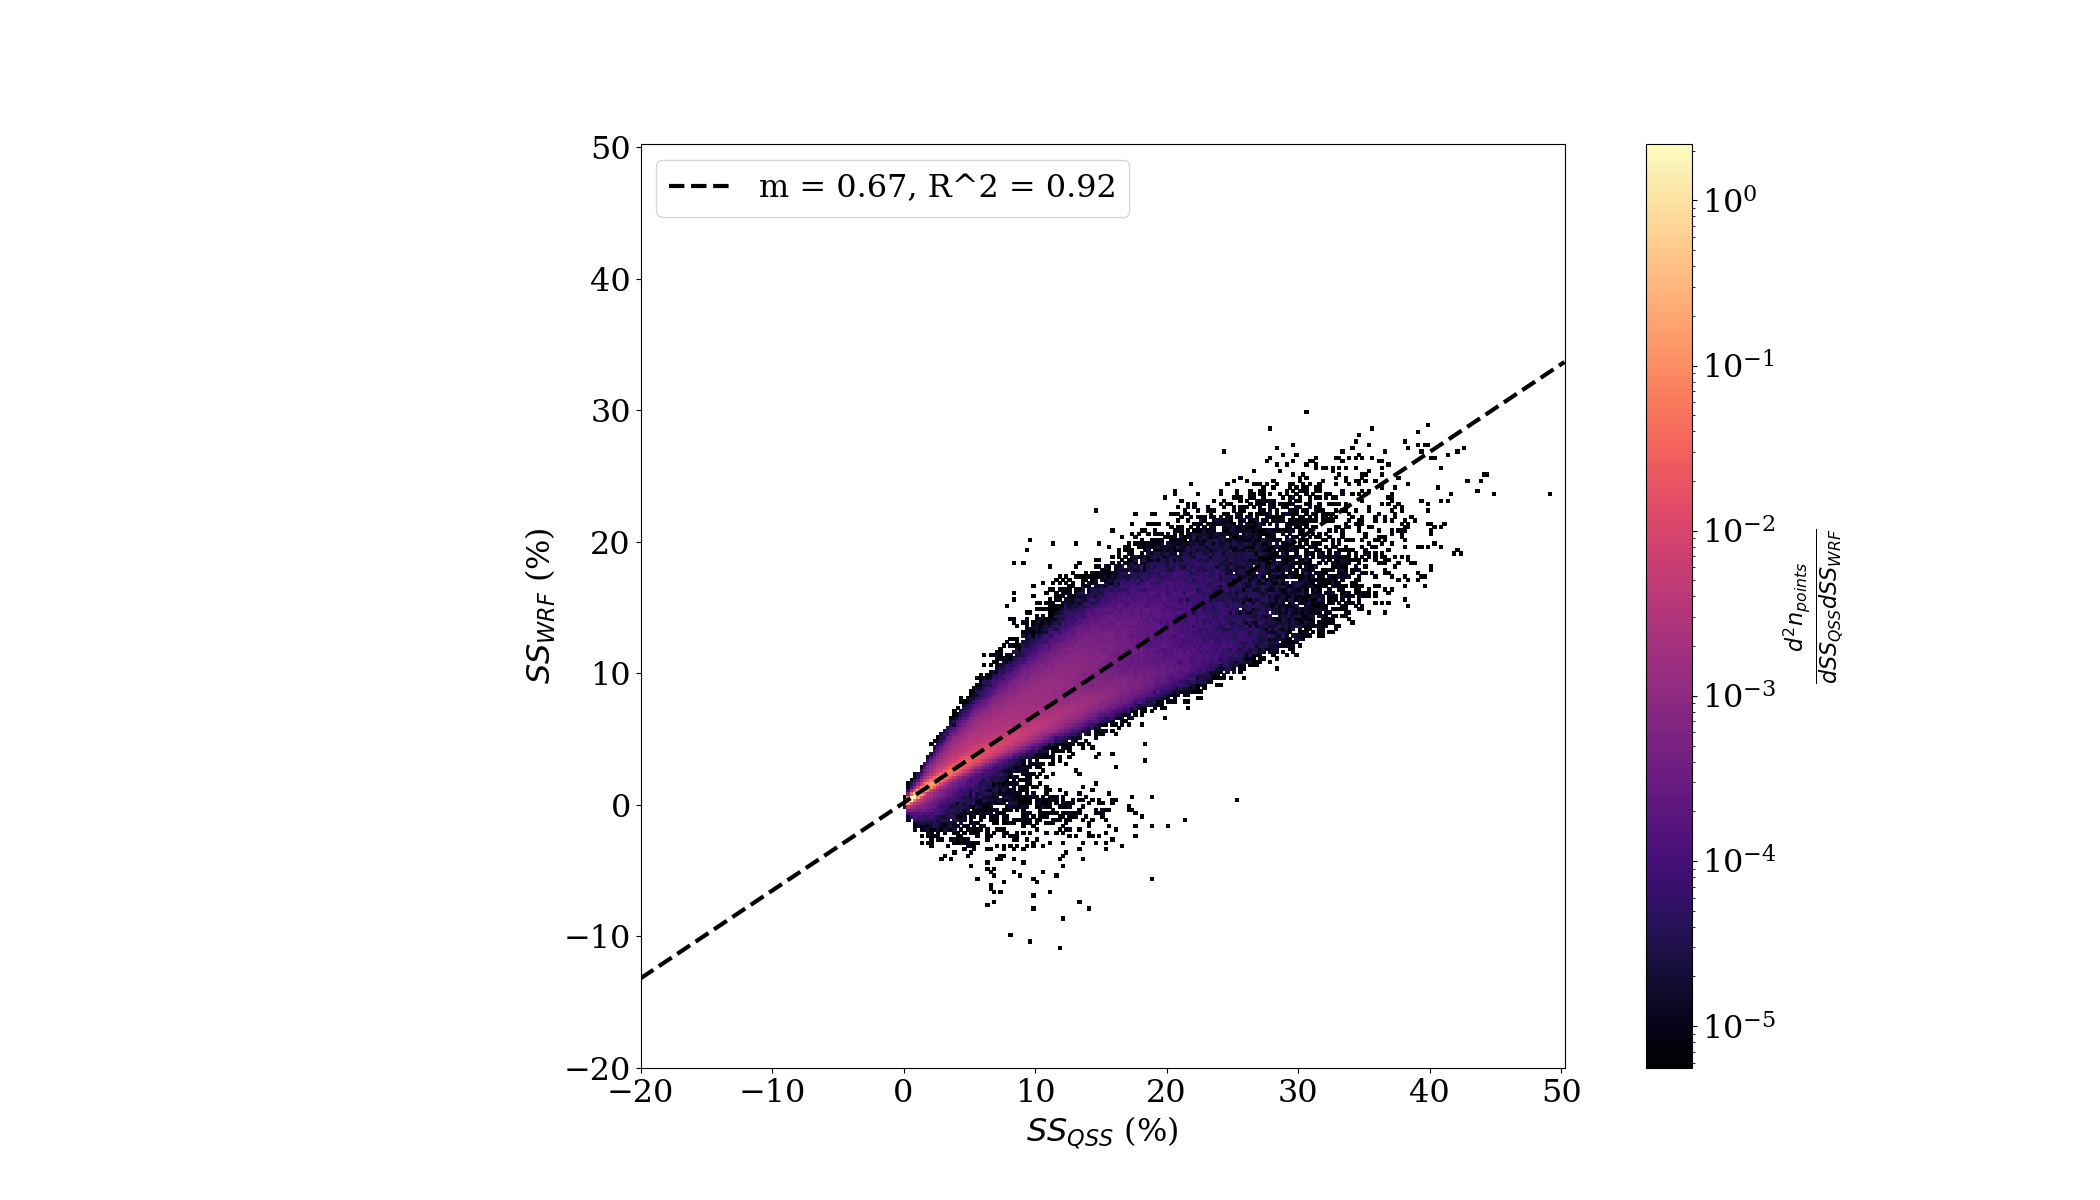
\includegraphics[width=\textwidth]{revmywrf/v2_FINAL_heatmap_ss_qss_vs_ss_wrf_Unpolluted_figure.png}
		\caption{Unpolluted case.}
		\label{wrfvsqssunpollv2}
	\end{subfigure}
	\begin{subfigure}{0.7\textwidth}
		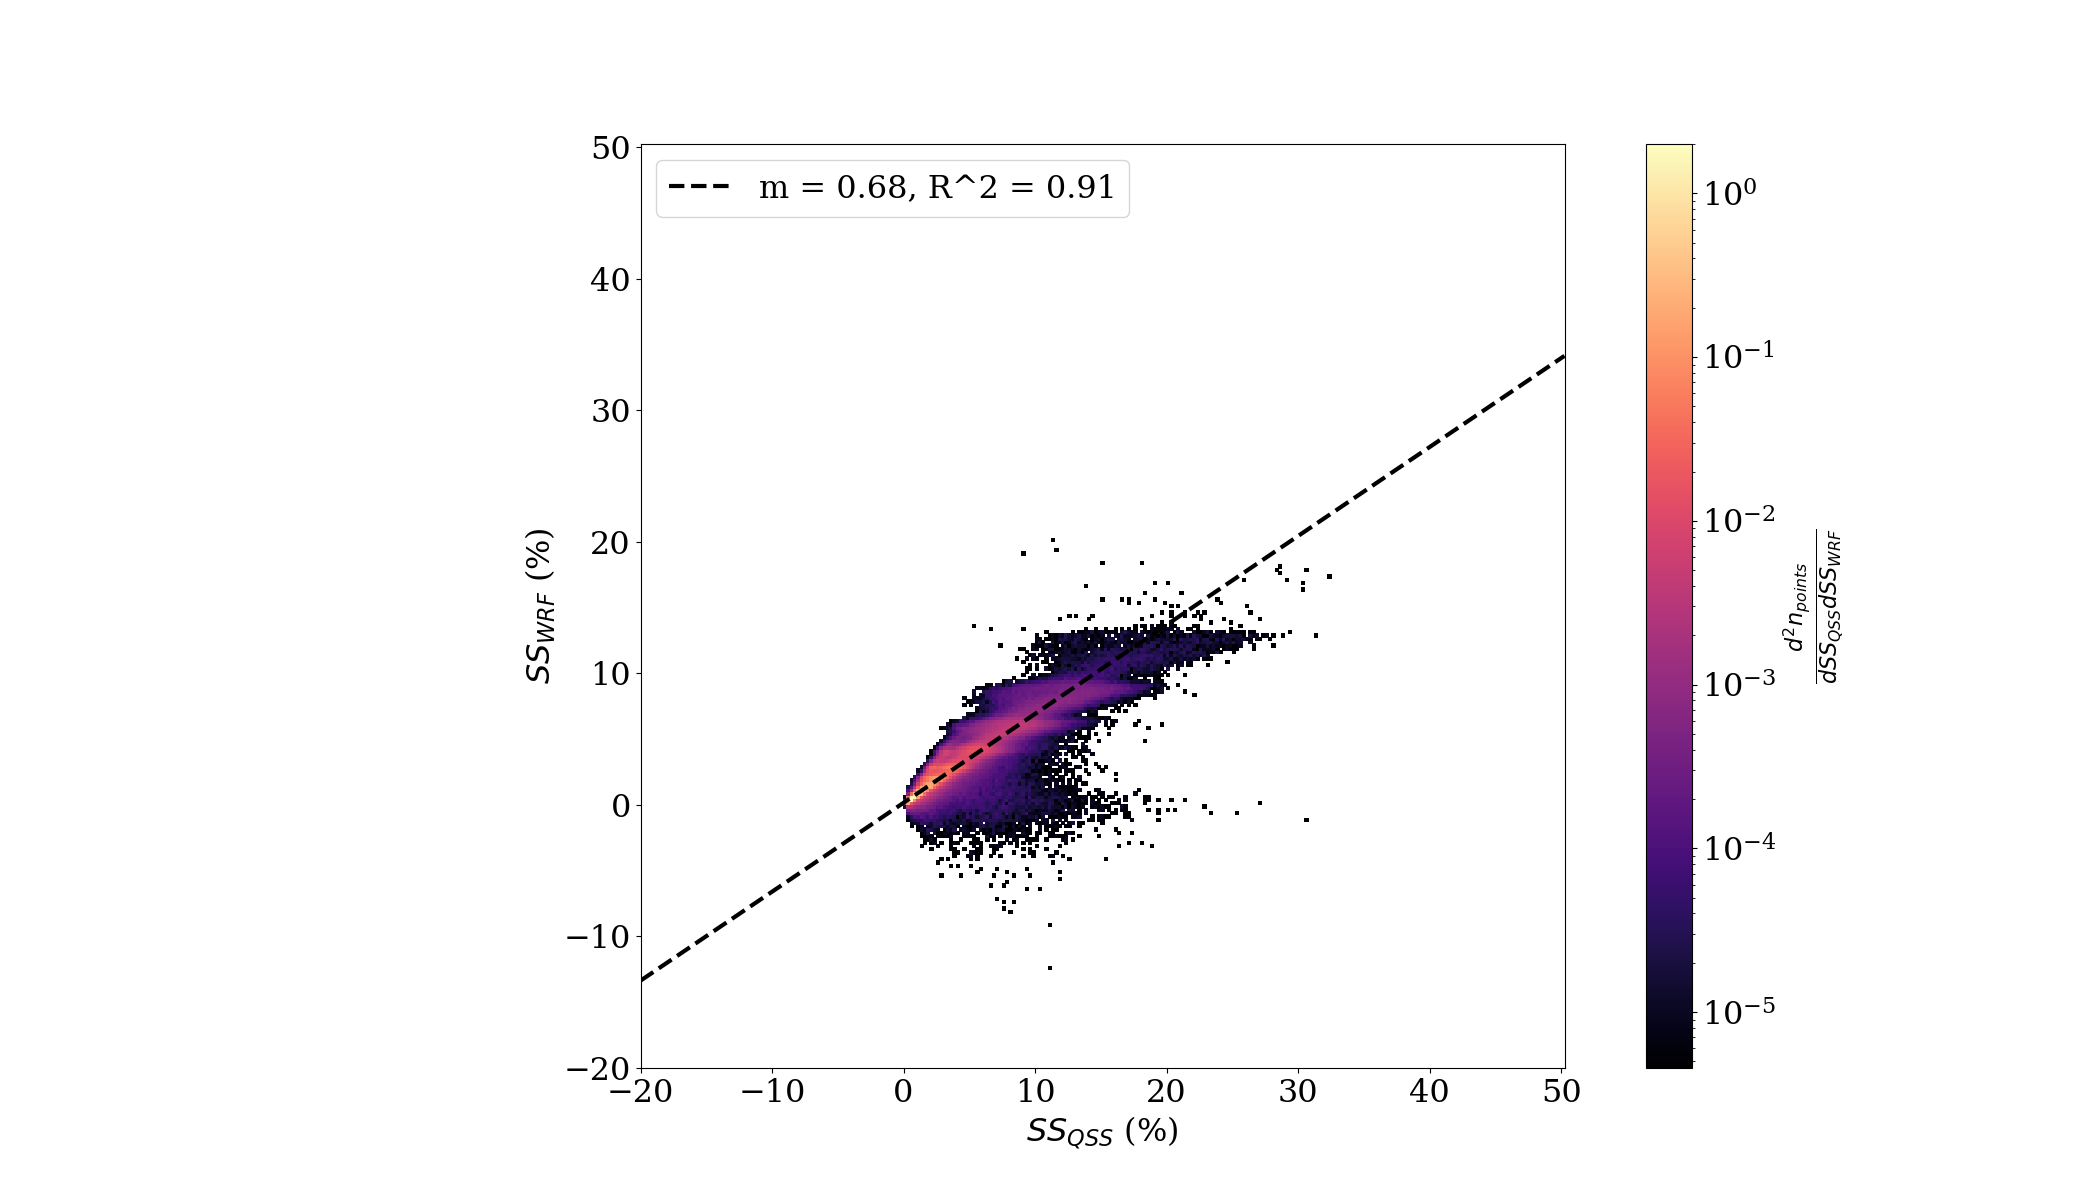
\includegraphics[width=\textwidth]{revmywrf/v2_FINAL_heatmap_ss_qss_vs_ss_wrf_Polluted_figure.png}
		\caption{Polluted case.}
		\label{wrfvsqsspollv2}
	\end{subfigure}
	\caption{Actual ($SS_{WRF}$) vs predicted ($SS_{QSS}$) supersaturation, using simplified form of Equation \ref{fullss}. Color indicates density of data points; note the scale is logarithmic.}
	\label{wrfvsqssv2}
\end{figure}

We use the expressions given in \cite{Pruppacher2010} and \cite{Rogers1989} for ventilation corrections [ \klcomm{They are kind of extensive...should I write out all formulae or just refer to the code in GitHub?} ]. Figures \ref{wrfvsqssv3} and \ref{wrfvsqssv5} show, respectively, the effects of neglecting these corrections (i.e. setting $f(r)=1$ for all $r$) for rain drops (defined here as liquid water drops with diameter greater than 50 $\mu$m), and omitting rain drops altogether from the calculations of mean radius and number concentration.

\begin{figure}[ht]
	\centering
	\begin{subfigure}{0.7\textwidth}
		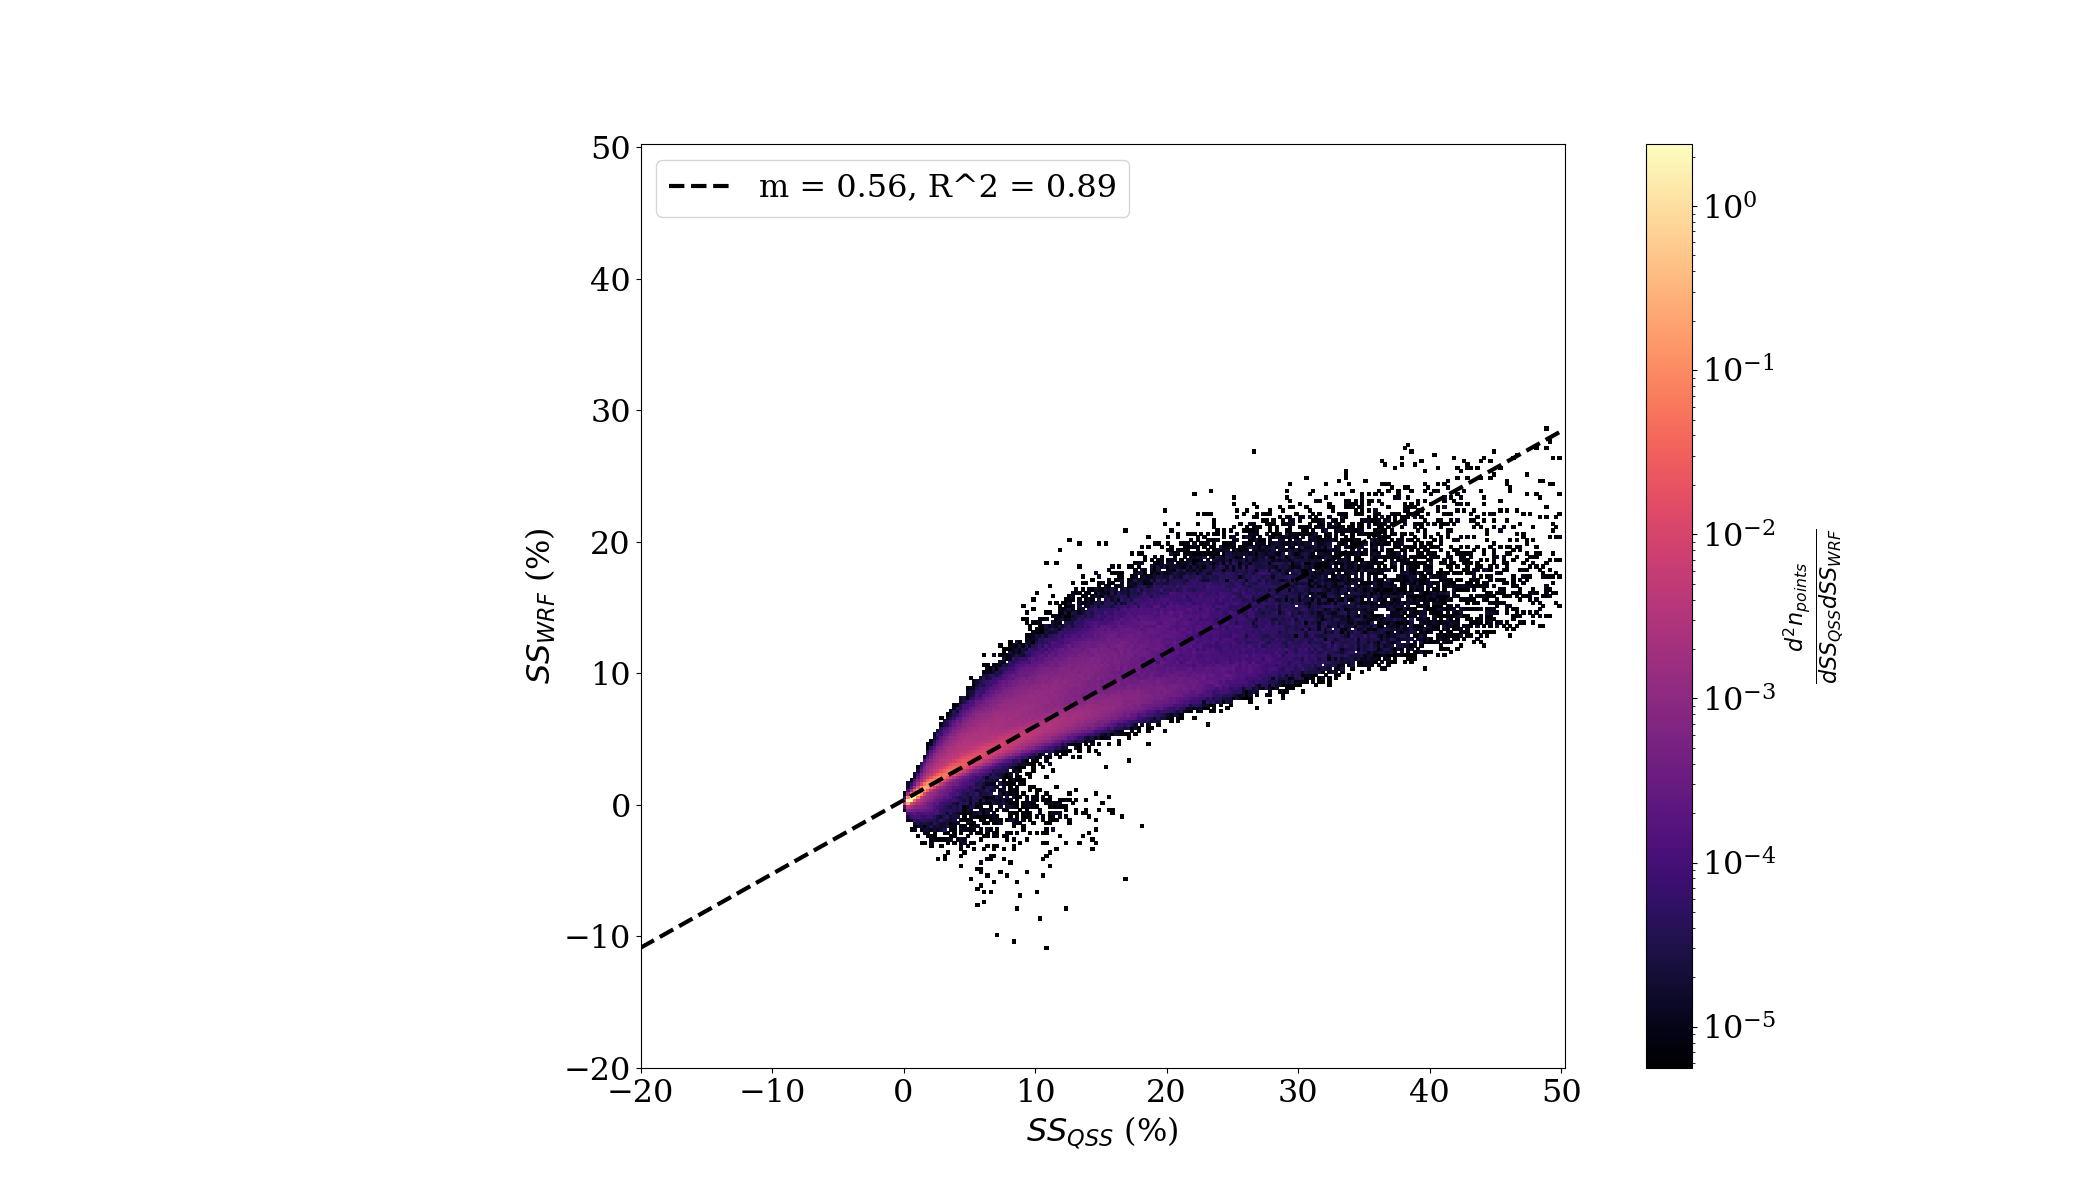
\includegraphics[width=\textwidth]{revmywrf/v3_FINAL_heatmap_ss_qss_vs_ss_wrf_Unpolluted_figure.png}
		\caption{Unpolluted case.}
		\label{wrfvsqssunpollv3}
	\end{subfigure}
	\begin{subfigure}{0.7\textwidth}
		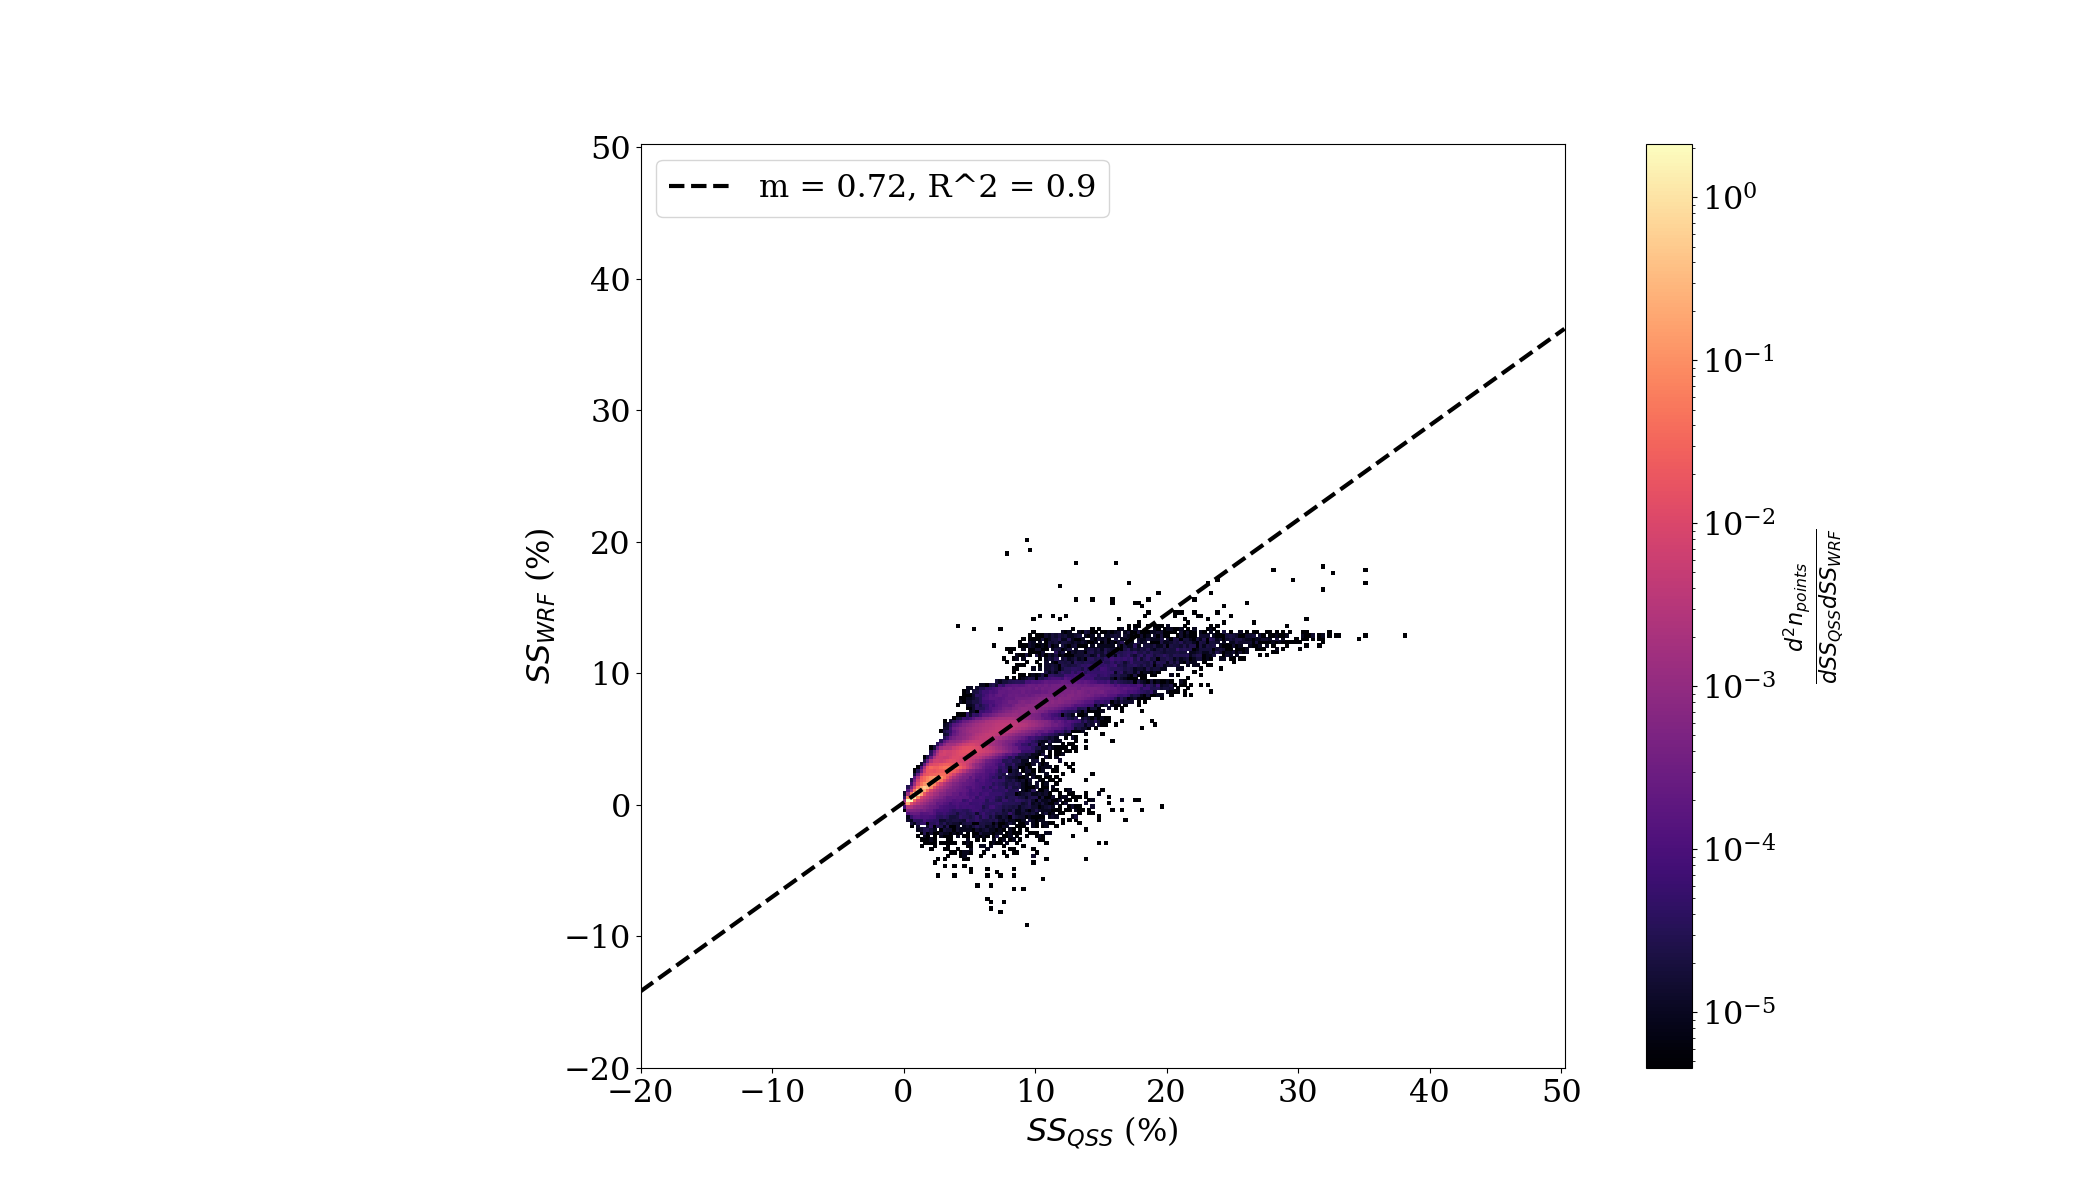
\includegraphics[width=\textwidth]{revmywrf/v3_FINAL_heatmap_ss_qss_vs_ss_wrf_Polluted_figure.png}
		\caption{Polluted case.}
		\label{wrfvsqsspollv3}
	\end{subfigure}
	\caption{Actual ($SS_{WRF}$) vs predicted ($SS_{QSS}$) supersaturation, without ventilation corrections. Color indicates density of data points; note the scale is logarithmic.}
	\label{wrfvsqssv3}
\end{figure}

\begin{figure}[ht]
	\centering
	\begin{subfigure}{0.7\textwidth}
		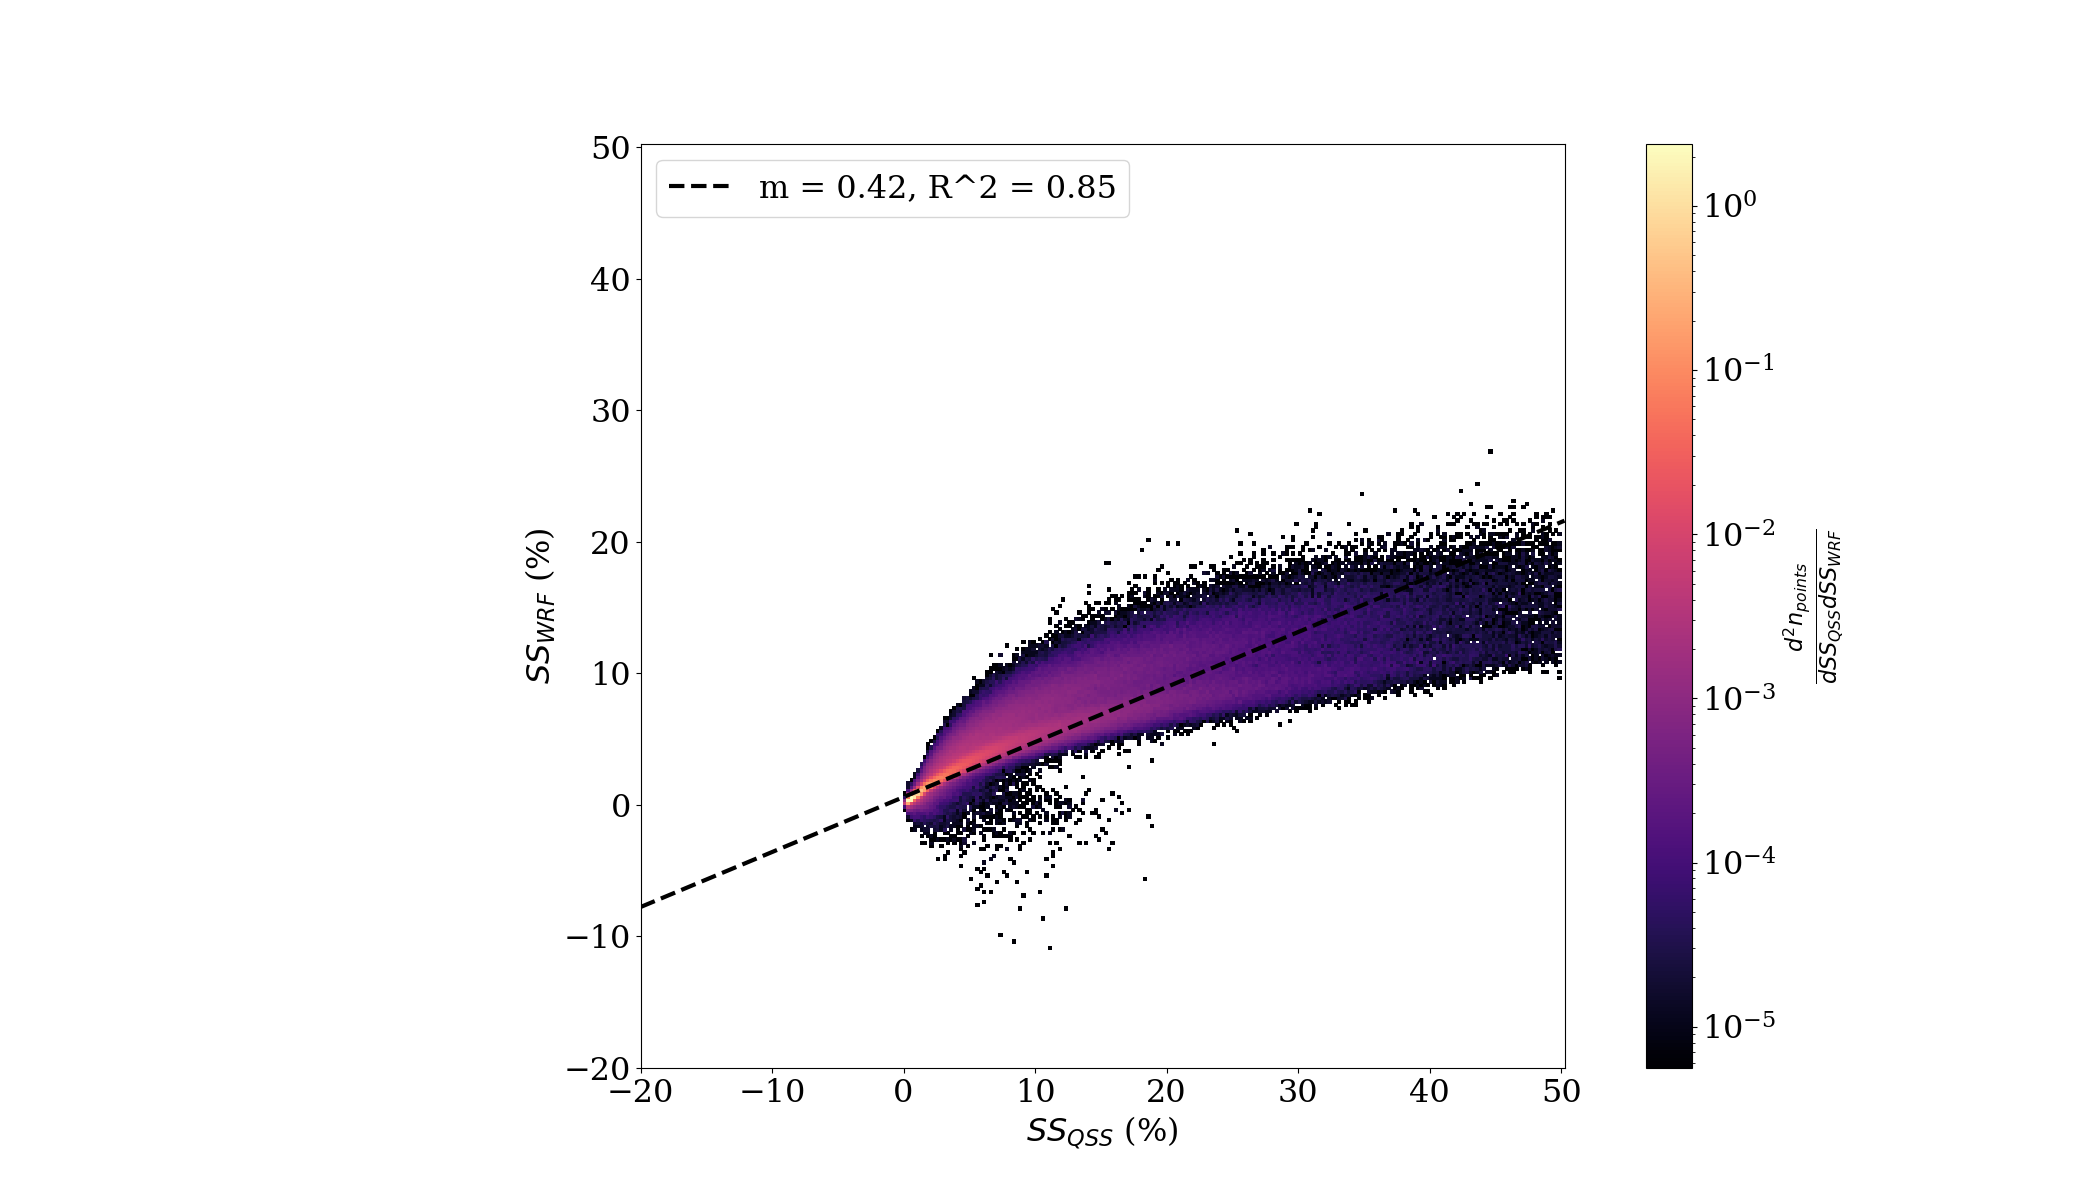
\includegraphics[width=\textwidth]{revmywrf/v5_FINAL_heatmap_ss_qss_vs_ss_wrf_Unpolluted_figure.png}
		\caption{Unpolluted case.}
		\label{wrfvsqssunpollv5}
	\end{subfigure}
	\begin{subfigure}{0.7\textwidth}
		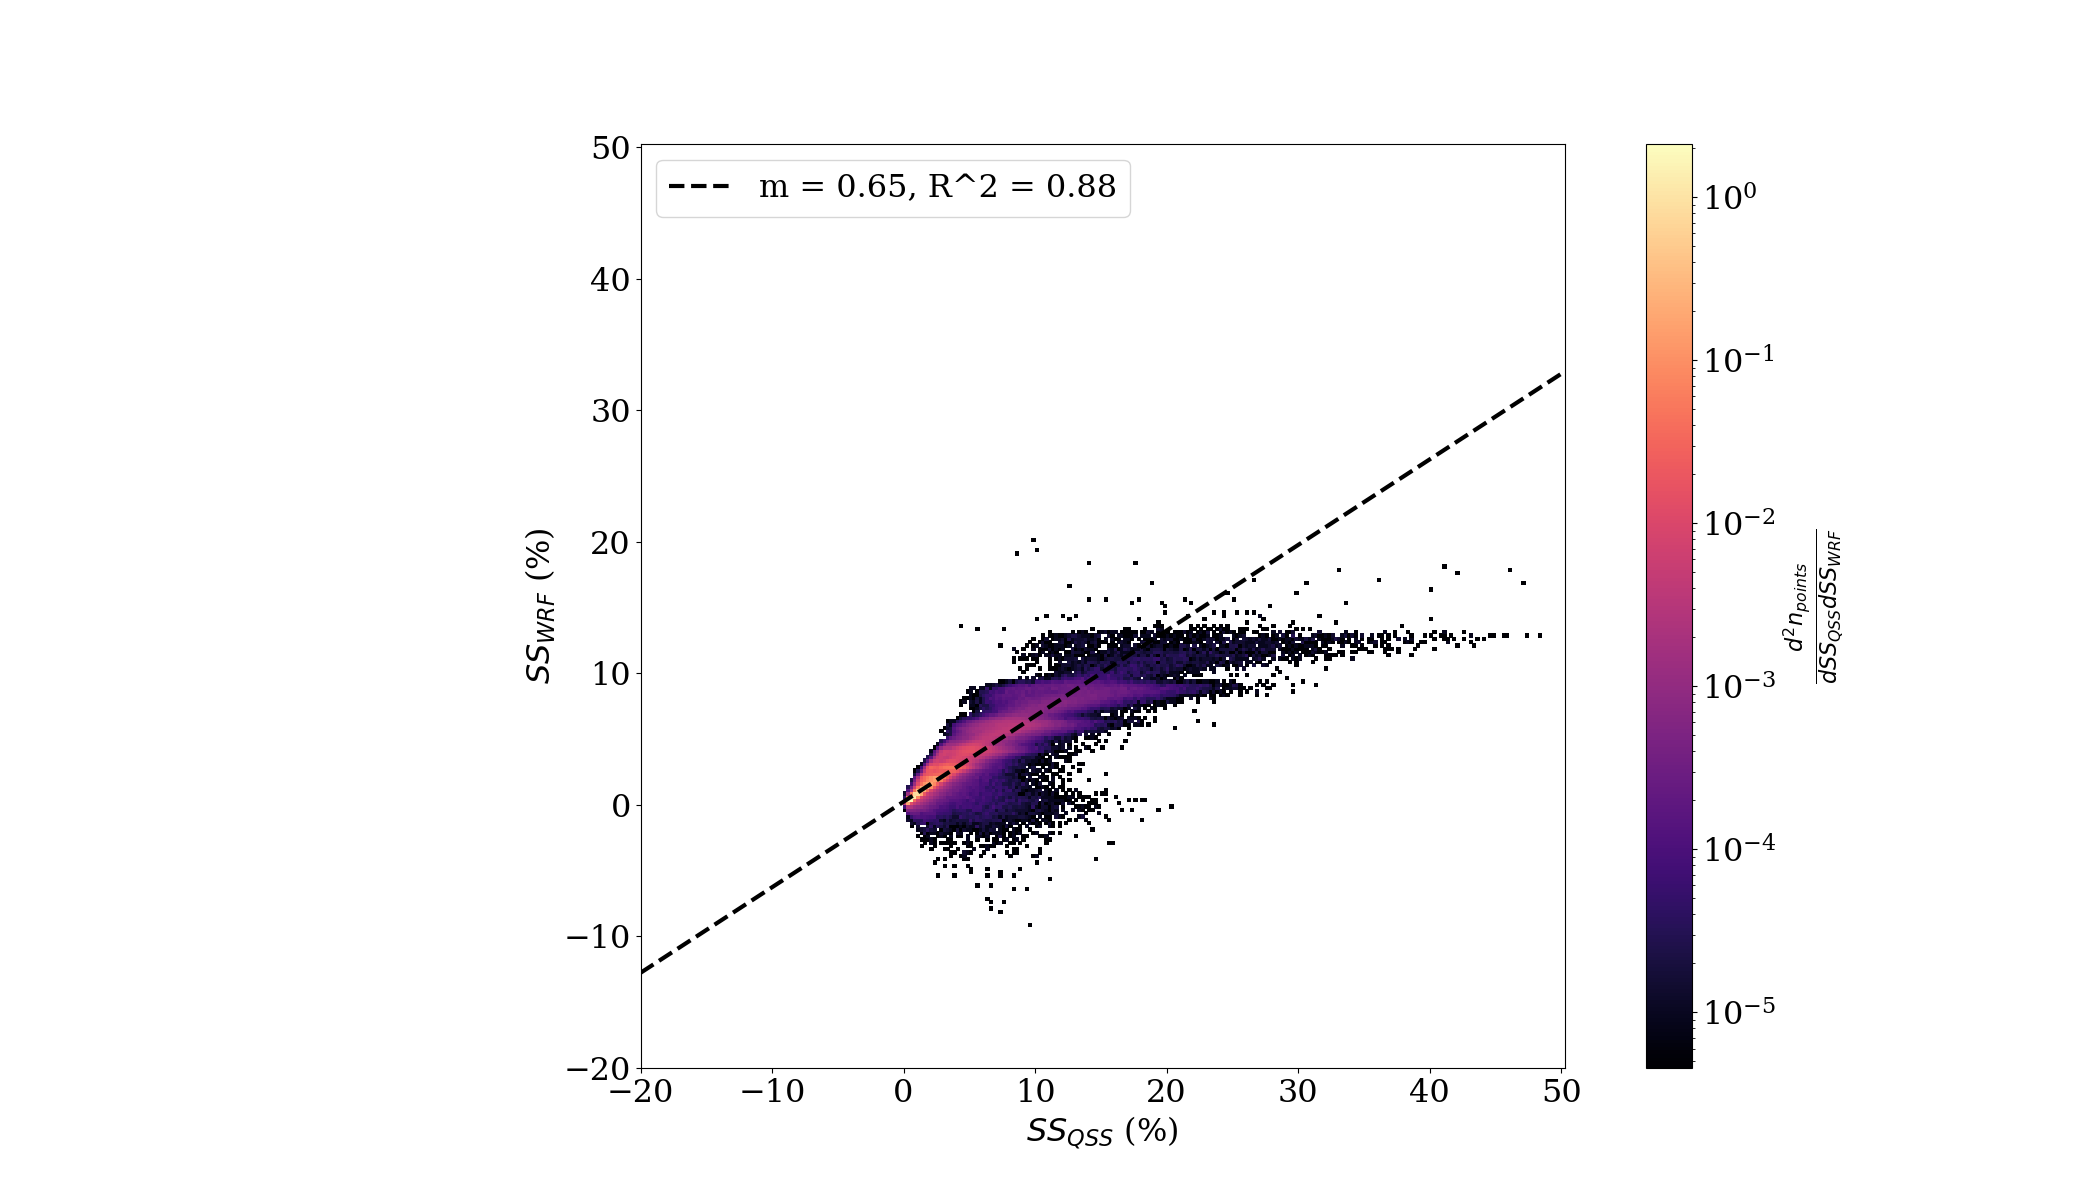
\includegraphics[width=\textwidth]{revmywrf/v5_FINAL_heatmap_ss_qss_vs_ss_wrf_Polluted_figure.png}
		\caption{Polluted case.}
		\label{wrfvsqsspollv5}
	\end{subfigure}
	\caption{Actual ($SS_{WRF}$) vs predicted ($SS_{QSS}$) supersaturation, without contributions from rain drops. Color indicates density of data points; note the scale is logarithmic.}
	\label{wrfvsqssv5}
\end{figure}

Finally, we note that we have excluded contributions to mean radius and number concentraiton from cloud droplets of diameter less than 5 $\mu$m, for consistency with our analysis of HALO data (see proceeding subsection). In the end this yields values for $SS_{QSS}$ which are indistinguishable to a reasonable number of significant figures.

\clearpage
\newpage

\subsection{HALO}

The HALO aircraft supported two instruments for measuring cloud droplet spectra: a cloud and aerosol spectrometer (CAS-DPOL) and a cloud droplet probe (one element of a cloud combination probe) (CCP-CDP) \cite{Braga2017}. We found that the CCP-CDP consistently reported unphysical bimodal size distributions, and therefore used only data from the CAS-DPOL for all calculations involving cloud droplets. Number concentrations from the CAS-DPOL were corrected using the $\xi$ factor derived in \cite{Weigel2016}.

The rain drop spectra came from data collected by greyscale cloud imaging probe (second element of the cloud combination probe) (CCP-CIP). The drop diameter detection ranges for CAS-DPOL and CCP-CIP were 0.89-50 $\mu$m and 25-2000 $\mu$m, respectively. Per guidance from the principal investigators for the CAS-DPOL, we only included data for droplets from size bins with a lower diameter bound greater than 3 $\mu$m in the analysis \cite{Jurkat2020}. Effectively (given size bins for this instrument), this meant that the lower bound on diameter for water drops was 5 $\mu$m. Because the CAS-DPOL and CCP-CIP have overlapping diameter detection ranges, we use concentrations for particles between 5 and 25 $\mu$m from CAS-DPOL and from 25 to 2000 $\mu$m from CCP-CIP. 

All measurements of environmental variables were taken from the Basic Halo Measurement and Sensor System (BAHAMAS).

Out of the dates for which all three instruments (BAHAMAS, CAS-DPOL, CCP-CIP) report data, we take those for which measurements of shared variables (true airspeed for BAHAMAS and CAS-DPOL; $\xi$ correction factor for CAS-DPOL and CCP-CIP) are well-correlated ($R^2$ above 0.95). These are (all in 2014): 6, 9, 11, 12, 16, 18, 27, 28, 30 September; 1 October.

We used the same Equation \ref{fullss} for $SS_{QSS}$ and for ventilation factors as described above.

\subsection{CAIPEEX}

Cloud droplet spectra for phase 1 of the CAIPEEX field campaign were measured by a CDP (detection range 2-1562.5 $\mu$m). We used the data from the following flight dates in 2009: 16, 21, 22 June; and 18, 23, 24, 25 August.

We used the same Equation \ref{fullss} for $SS_{QSS}$ and for ventilation factors as described above, and excluded data from cloud droplets of diameter less than 5 $\mu$m.

\begin{figure}[ht]
	\centering
	\begin{subfigure}{0.7\textwidth}
		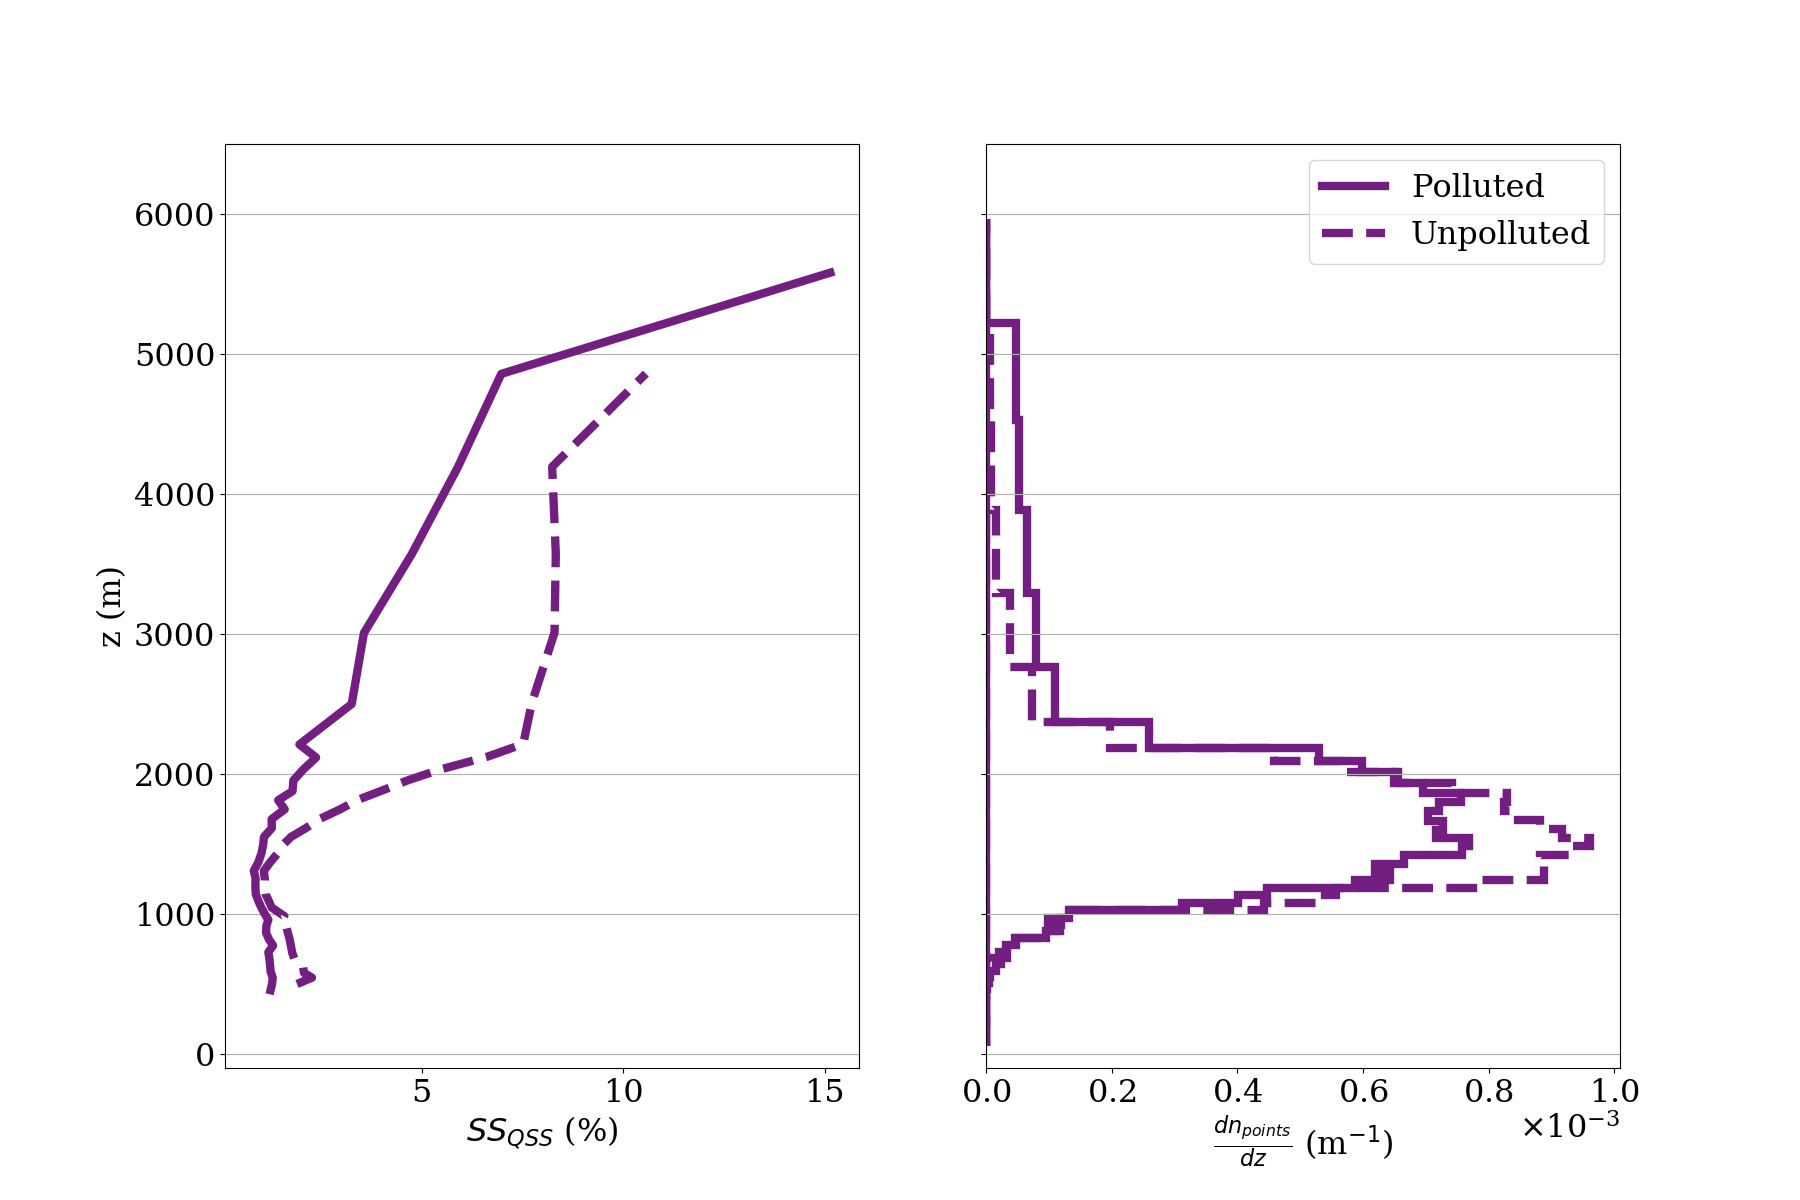
\includegraphics[width=\textwidth]{revmywrf/v2_FINAL_subdom_bipanel_ss_qss_vs_z_allpts_figure.png}
		\caption{}
		\label{wrfsubdombipanelallpts}
	\end{subfigure}
	\begin{subfigure}{0.7\textwidth}
		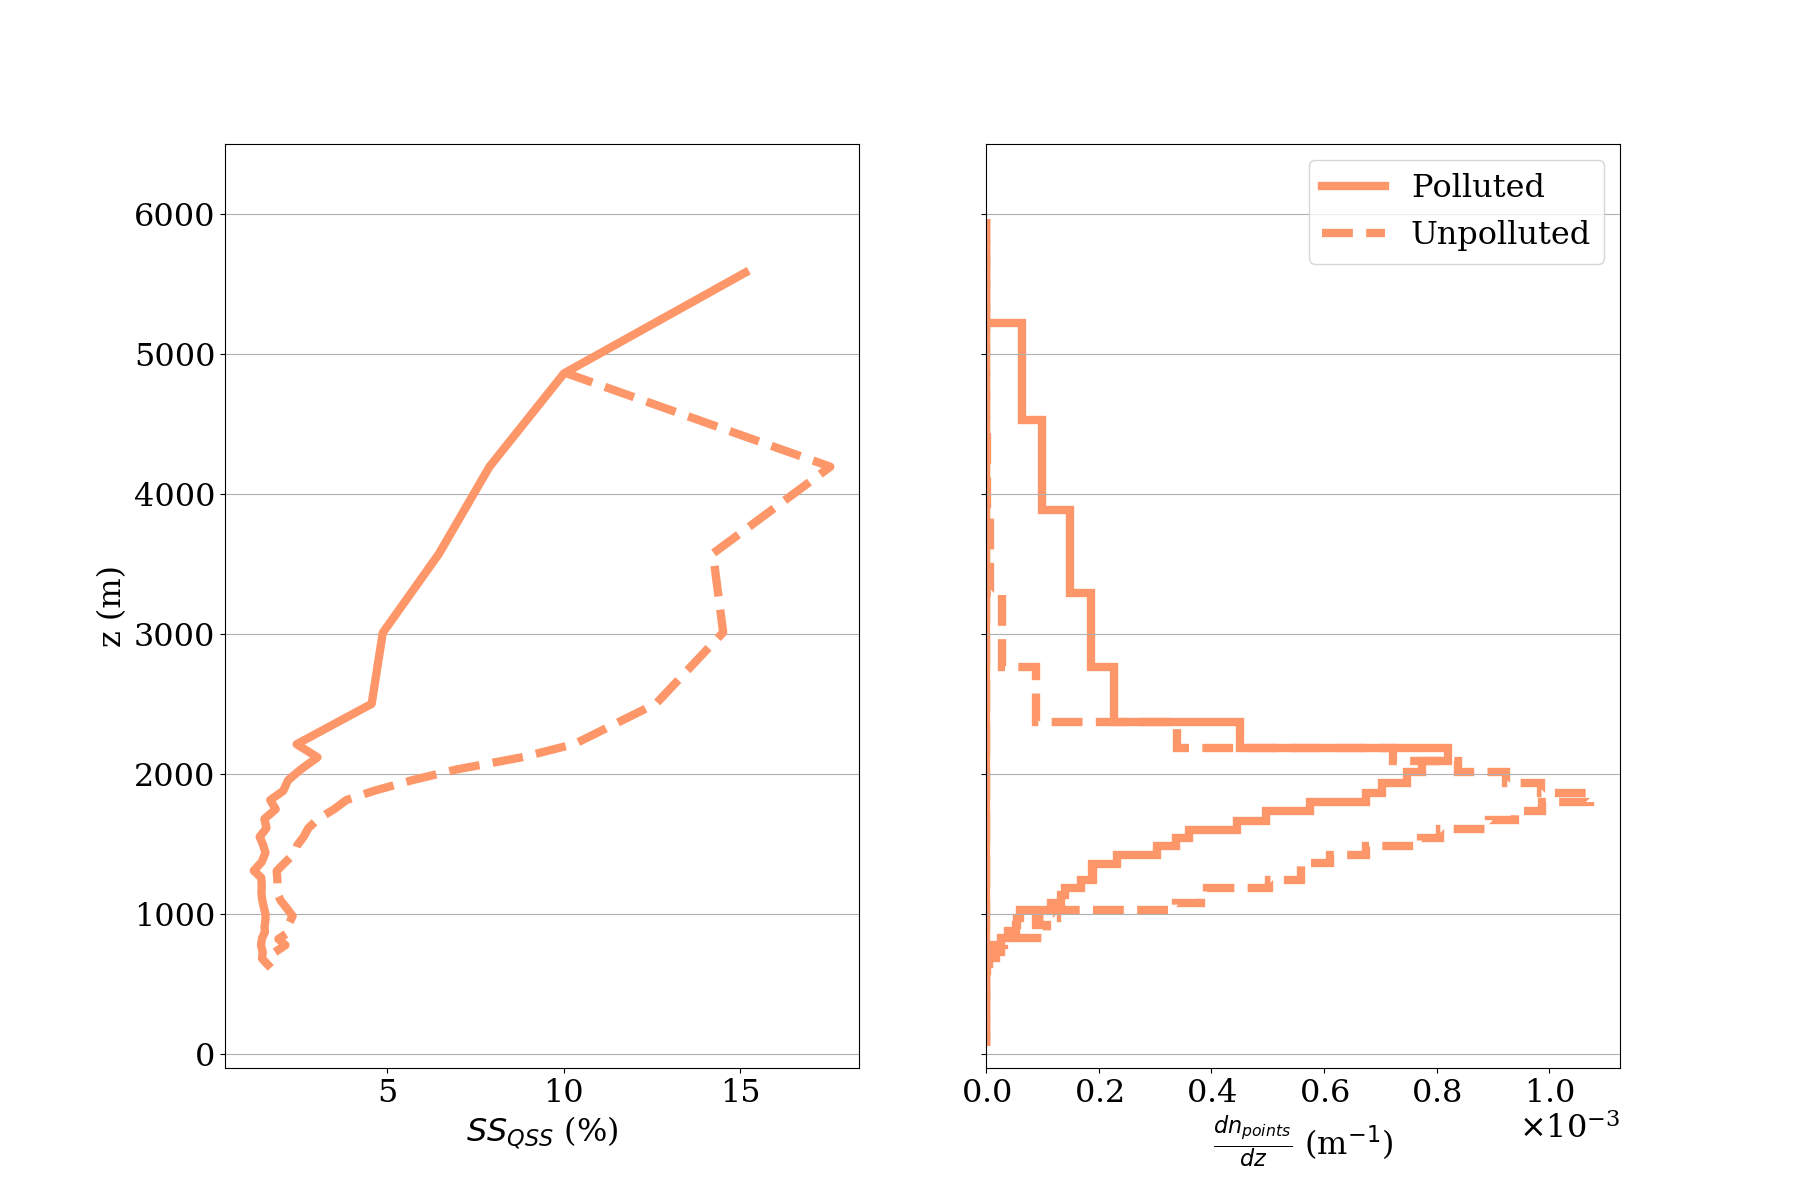
\includegraphics[width=\textwidth]{revmywrf/v2_FINAL_subdom_bipanel_ss_qss_vs_z_up10perc_figure.png}
		\caption{}
		\label{wrfsubdombipanelup50perc}
	\end{subfigure}
	\caption{Analagous to Figure \ref{wrfbipanel} restricted to the horizontal subdomain indicated by the red box in Figure S8 (bottom left panel).}
	\label{wrfsubdombipanel}
\end{figure}

\begin{sidewaystable}[]
\centering
\begin{tabular}{@{}llll@{}}
\toprule
Symbol & Meaning & Value of constant & Notes \\ \midrule
$C_{ap}$ & Specific heat capacity at constant pressure, dry air & 1005 J/kg &  \\
$D$ & Molecular diffusion constant of water in dry air & 0.23e-4 m$^2$/s & We take as constant wrt T \\
$e_s$ & Saturation vapor pressure, water & - &  \\
$f(r)$ & Ventilation factor & - &  \\
$g$ & Gravitational acceleration on Earth & 9.8 m/s &  \\
$K$ & Coefficient of thermal conductivity in dry air & 2.4e-2 J/(m s K) & We take as constant wrt T \\
$LWC$ & Liquid water content & - &  \\
$L_v$ & Latent heat of vaporization, water & 2.501e6 J/kg & We take as constant wrt T \\
$N$ & Particle number concentration & - &  \\
$n_{points}$ & Point number density & - & Used for heatmap figures \\
$q_v$ & Water vapor mass mixing ratio & - & Equals $\frac{m_v}{m_{tot}}$ \\
$q_v^*$ & Saturation water vapor mass mixing ratio & - & Equals $\frac{m_v^*}{m_{tot}}$ \\
$r$ & Particle radius & - &  \\
$RH$ & Relative humidity & - & Equals $SS+1$ \\
$\rho_a$ & Mass density, dry air & - & Assuming ideal gas law \\
$\rho_w$ & Mass density, liquid water & 1000 kg/m$^3$ &  \\
$R_a$ & Ideal gas constant, dry air & 287.19 J/(kg K) &  \\
$R_v$ & Ideal gas constant, water & 460.52 J/(kg K) &  \\
$SS$ & Supersaturation & - & Equals $RH-1$ \\
$T$ & Temperature & - &  \\
$T_c$ & Temperature in degrees C & - & Equals $T – 273.15$ \\
$w$ & Vertical wind velocity & - &  \\
$z$ & Altitude & - &  \\ \bottomrule
\end{tabular}
\caption{Explanation of constants and variables used in the paper.}
\label{vartable}
\end{sidewaystable}

\clearpage
\newpage

\bibliography{refs}
\bibliographystyle{ieeetr}
\end{document}
